\documentclass{article}
\usepackage[a4paper, top=2cm, bottom=2cm, left=2cm, right=2cm]{geometry}

\usepackage{hyperref} % For the Table of Contents
\usepackage{enumitem} % For lists

\usepackage{graphicx}
\usepackage{float} % ← serve per [H]

\usepackage{xcolor}
\usepackage{minted}

\newminted[mypython]{python}{
  linenos,
  fontsize=\small,
  frame=leftline,
  framesep=4mm,
  baselinestretch=1.2,
  breaklines=true,
  tabsize=4,
  escapeinside=||,
  style=paraiso-light
}

\title{Comparative Analysis of Selection Algorithms}

\author{University of Udine\\Department of Mathematical, Computer and Physical Sciences}
\date{2024/05/26}
\begin{document}

\maketitle

% Table of Contents (acts as your index)
\tableofcontents
\newpage

\section{Introduction}

\subsection{Project Purpose}
The project focused on the implementation of three different algorithms to select the $k$-$th$ smallest element in an array, given $k$, and on the comparative analysis of the behaviour of these algorithms in the average case.\\
It also focused on the implementation of a $benchmark$ that was able to accurately measure the performance of the three algorithms and generate a graph on a logarithmic scale that effectively represented their performance as the size of the arrays used and the choice of the $k$ parameter varied.

\subsection{Project Team and Responsibilities}
This project was developed by a team of three university students: \\ \\
\begin{minipage}{\linewidth} \centering
    \begin{tabular}{|c|c|} 
        \hline \textbf{Name} & \textbf{University Mail} \\ \hline 
        Francesco Verrengia & 157847@spes.uniud.it \\ \hline
        Martina Ammirati & 161831@spes.uniud.it \\ \hline
        Riccardo Gottardi & 162077@spes.uniud.it \\ \hline
    \end{tabular}
\end{minipage} 
\\ \\
In this project, Francesco Verrengia was primarily responsible for:
\begin{itemize}
    \item \textbf{General Project Management}: Oversaw code version control and coordinated task distribution.
    \item \textbf{Algorithm Implementation}: Co-developed the component of the $bench$-$mark$ responsible for measuring execution times.
    \item \textbf{Graph Generation}: Implemented the code for automated graph creation.
\end{itemize}
In this project, Martina Ammirati was primarily responsible for:
\begin{itemize}
    \item \textbf{Algorithm Implementation}: Developed the $QuickSelect$ and $Median$ $OfMedians$ algorithms.
    \item \textbf{Document Preparation}: Translated the full report from Italian to English, maintaining technical precision; additionally, converted the original draft (in Obsidian) into a formatted LaTeX document.
    \item \textbf{Graph Generation}: Redesigned the graph-generation module to follow a modular architecture, enabling easy extension or reuse in future analyses.
    
\end{itemize}
In this project, Riccardo Gottardi was primarily responsible for:
\begin{itemize}
    \item \textbf{Algorithm Implementation}: Developed the $HeapSelect$, $QuickSort3$-$Way$ and $QuickSort3WayRandomized$ algorithms.
    \item \textbf{Algorithm Implementation}: Co-developed the component of the $bench$-$mark$ responsible for measuring execution times.
\end{itemize}

\subsection{Selection Algorithms Used}
Selection algorithms, such as the ones used in this analysis, are used to find the $k$-$th$ smallest (or largest) element in a data set without having to sort the entire data set. This type of operation is crucial in various areas of computer science and applied mathematics. \\
In statistics, for example, finding the median or other percentiles of a data set is essential. The median is often used as a central measure that is resistant to outliers, while percentiles describe the distribution of the data. Selection algorithms allow these measures to be computed efficiently.\\
In machine learning, during the data preprocessing phase, selecting the median or other sorted elements can help normalize the data, making it easier to analyse. A common normalization method is median normalization, in which selection algorithms play a key role.\\
These algorithms are also widely used in computer graphics and in the optimization of sorting algorithms, such as $QuickSort$.

\subsection{Languages and Libraries}
We chose to structure the entire project in $Python$ because, although it is slower than languages such as $C$ and $C++$, it offers a very simple syntax.\\
This choice favour the readability of the code, which was our main prerogative for this project.\\
Also, for readability reasons, all the procedures called by the 3 main algorithms and by $benchmark$ are included in the dedicated 'Appendix' sections and were not included in the sections relating to the individual algorithms.\\
For the selection algorithms, no external libraries were used.\\
However, for $benchmark$, the following libraries were used: $random$, $time$, $os$, $matplotlib$.

\subsection{Tools Used}
The $benchmark$ was run in a controlled environment, on a standard 2020 Macbook Air M1, and no other programs were running during its execution.
\begin{itemize}
    \item CPU: $AppleM1$
    \item RAM: 8GB
    \item SSD: 250GB
    \item Operating System: $macOS$ $Sonoma$ 14.5
\end{itemize}
Note that the $benchmark$ was also tested on a laptop running $Ubuntu$ $22.04.4LTS$ and was not intended to run on $Windows$.
In particular, the execution times on $Windows$ were extremely high, probably due to the use of the $time.monotonic()$ function; moreover, in the case of execution on $Windows$, the graph would not be generated.

\section{The Algorithms}
\subsection{Quick Select}
In the (iterative) version of $QuickSelect$ implemented, during the search phase for the $k$-$th$ element, the call to $partition$ was iterated on subsets of the array of increasingly smaller size until the pivot on which the partition was performed coincided with the $k$-$th$ element or the subarray considered was of unit size.\\
In fact, the complexity of the algorithm was due almost entirely to $Partition$, whose task was to partition the array using a pivot in the following manner: It had to move all the elements smaller than the pivot to its left and all the larger ones to its right, ending with the pivot in the position in which it would be if the array were sorted.\\
After the call to $Partition$:\\
- If $k$ was smaller than the pivot, the call was iterated on the array partition containing the elements smaller than the pivot.\\
- If $k$ was greater than the pivot, it was iterated on the partition that contained the larger elements.\\
Otherwise, the pivot was the $k$-$th$ element, so $Partition$ ended with the return of the pivot.\\
In the best case, $Partition$ was called $\Theta(1)$ times, so $QuickSelect$ had, as the best complexity, $\Theta(n)$.\\
The worst case for $QuickSelect$ was when the array was sorted in ascending order and was asked to find an element whose position $k$ was close to the beginning of the array.\\$Partition$ would then run on an array partition that decreased by exactly one element each time. It would therefore perform about $n^2/2$ operations, so $QuickSelect$ would then have a complexity of $\Theta(n^2)$. \\ 
In general, we can say that $QuickSelect$ has a time complexity O$(n^2)$. \\
Figure 1 was generated with arrays sorted in ascending order, $k=1$ and $testForEachN = 20$ instead of $500$ because the benchmark execution time in that case would have been significantly higher. Also, by fixing $k$, and using always sorted arrays, the performance variability was significantly reduced, so there was no need to run so many $testForEachN$.\\
Note: for the array of 100000 elements, the average execution time was 388.44495 69665987 seconds.

\begin{figure}[H]   
  \makebox[\textwidth][c]{%
    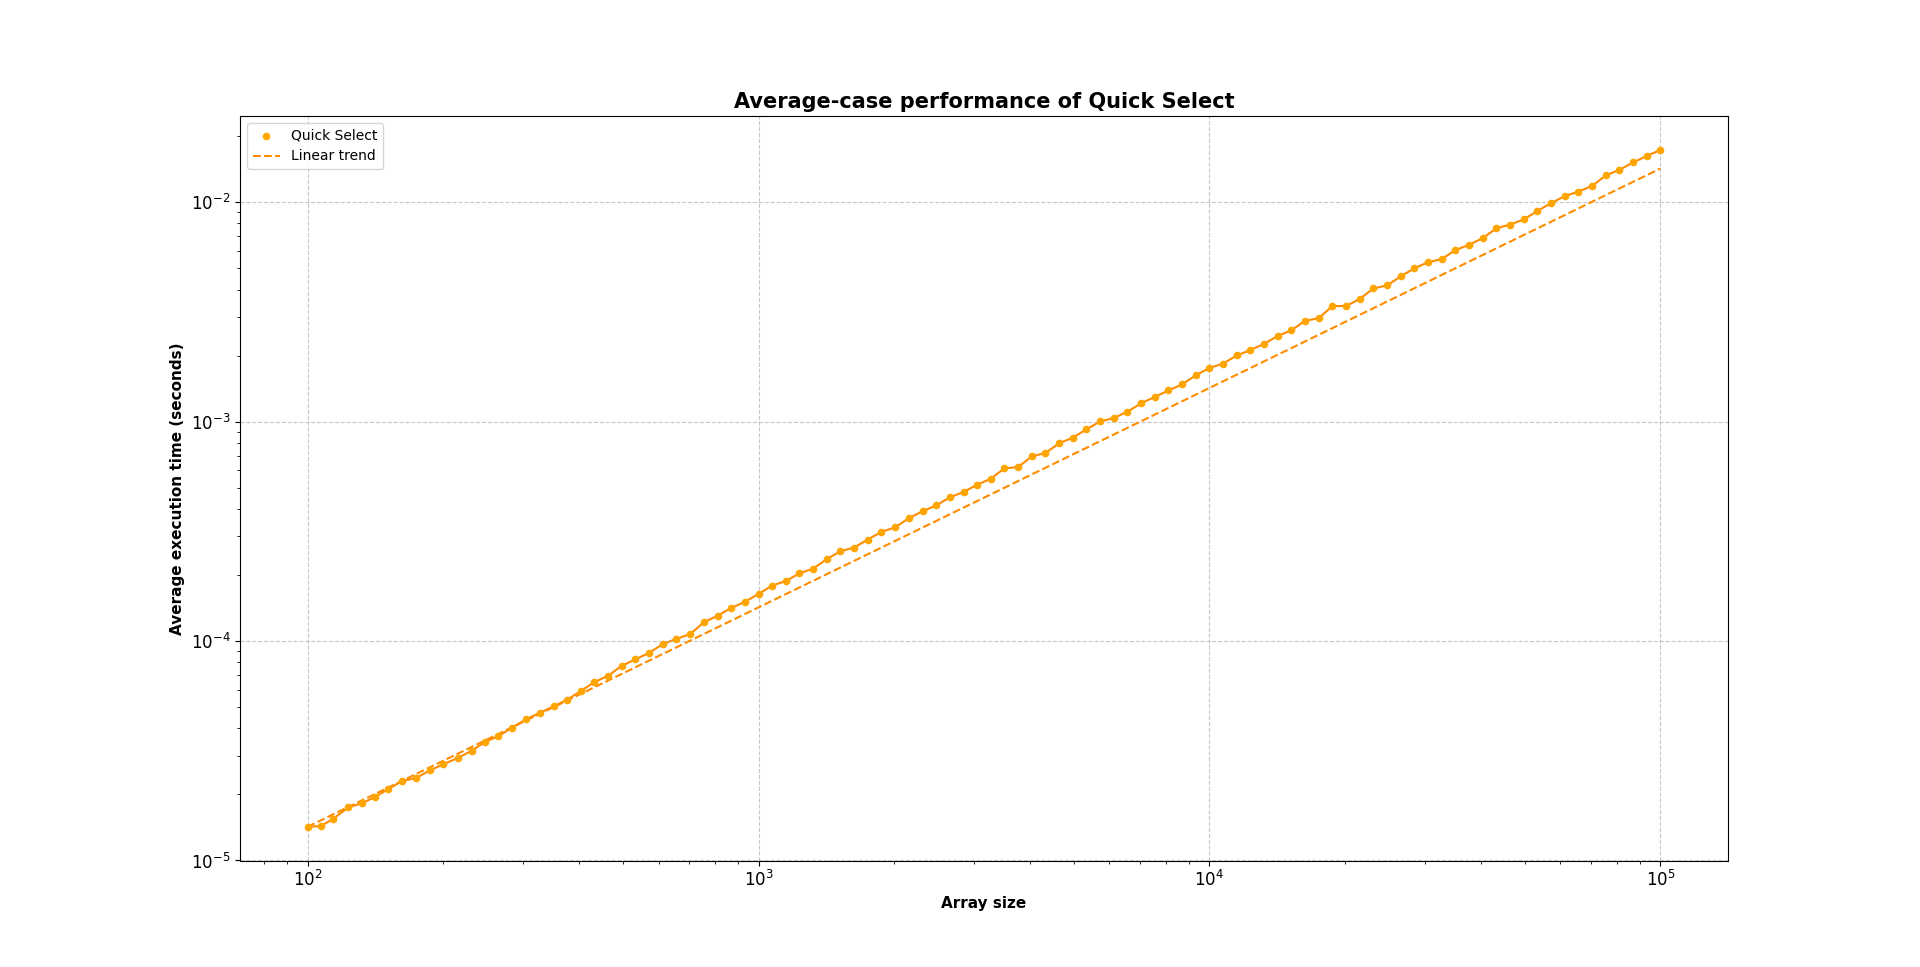
\includegraphics[width=1.2\textwidth]{Graphs/Quick Select/kIsRandom_Log.png}
  }
  \caption{Average-case performance of Quick Select - Logarithmic}
\end{figure}

\begin{figure}[H]   
  \makebox[\textwidth][c]{%
    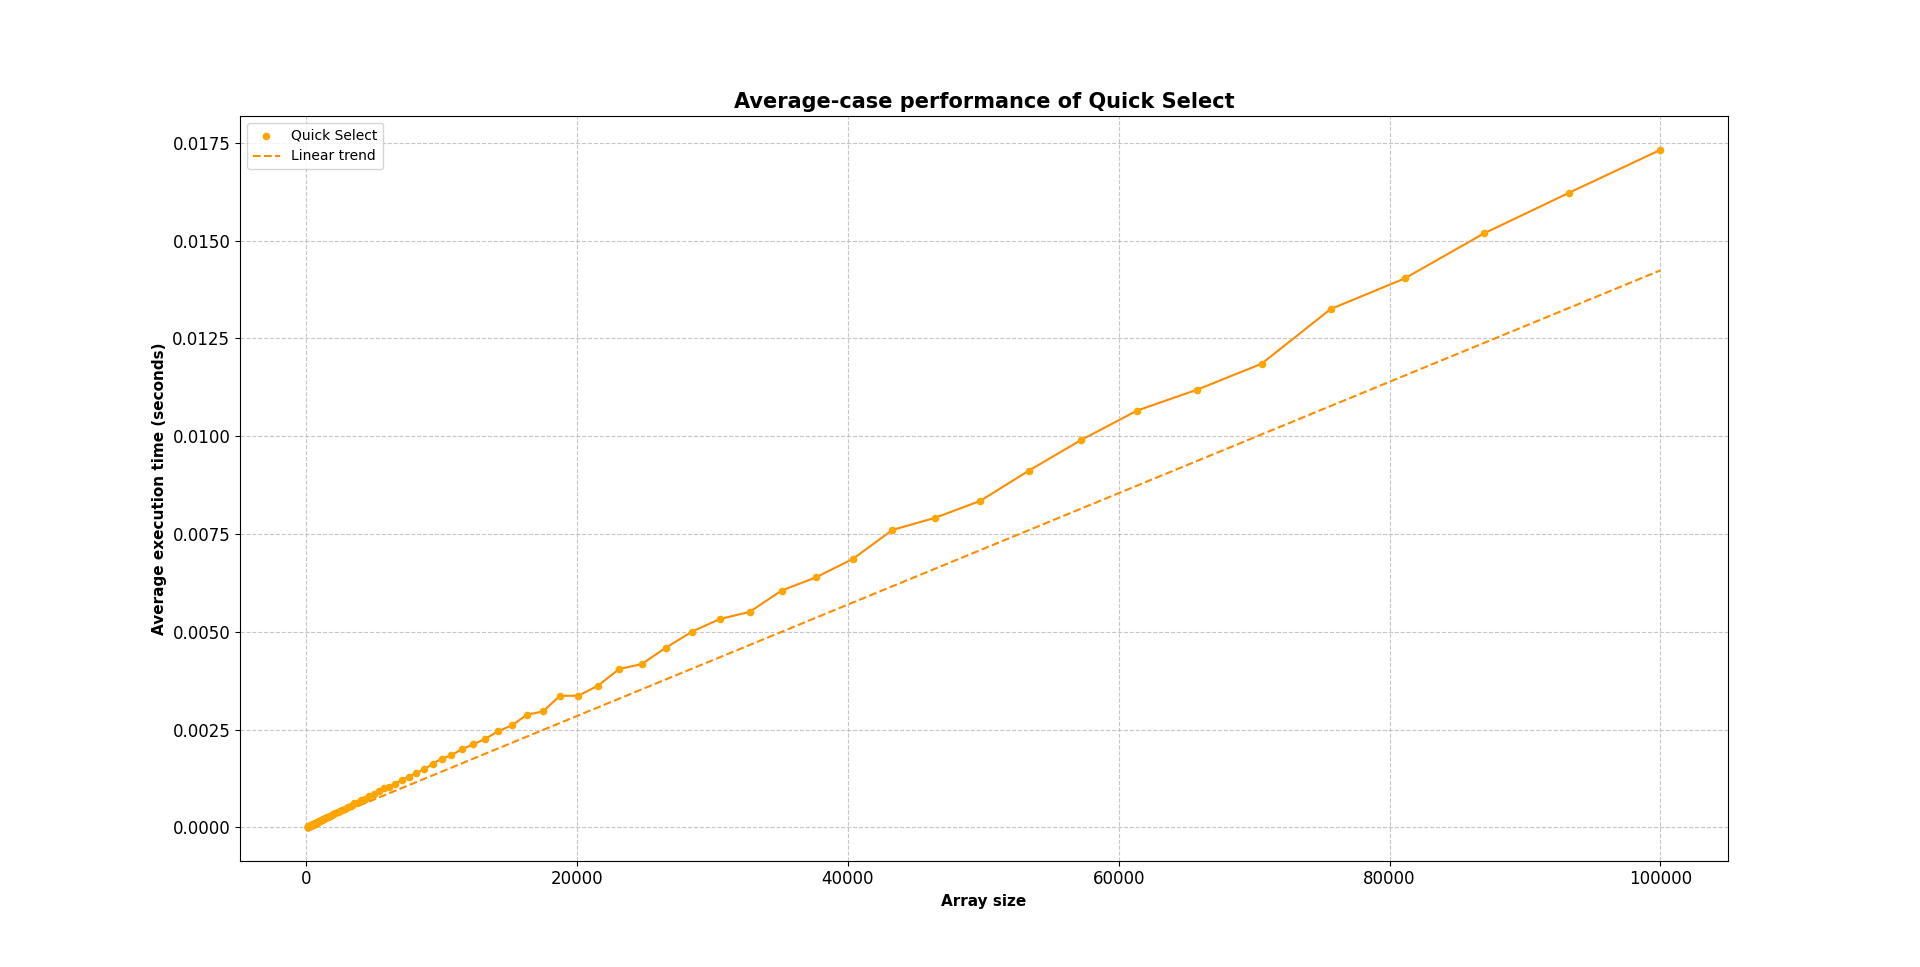
\includegraphics[width=1.2\textwidth]{Graphs/Quick Select/kIsRandom_notLog.png}
  }
  \caption{Average-case performance of Quick Select - Linear}
\end{figure}
\begin{figure}[H]   
  \makebox[\textwidth][c]{%
    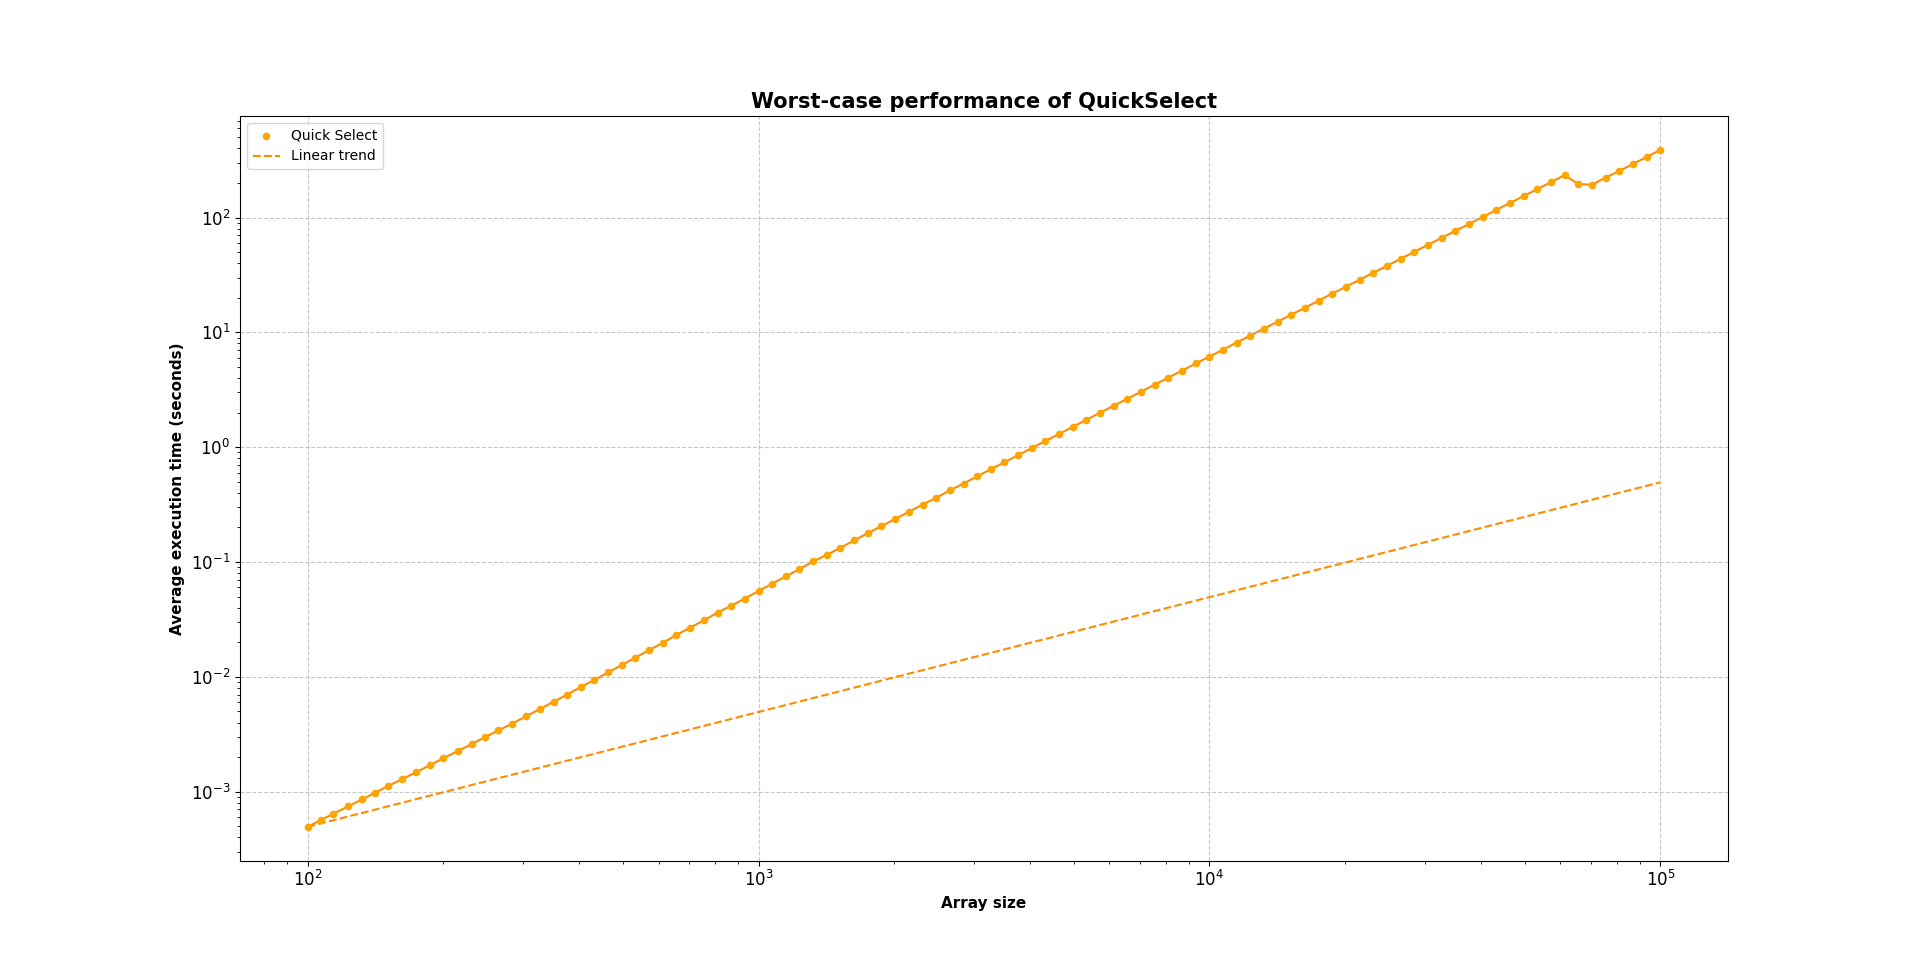
\includegraphics[width=1.2\textwidth]{Graphs/Quick Select/Worst_Log.png}
  }
  \caption{Worst-case performance of Quick Select - Logarithmic}
\end{figure}
\begin{figure}[H]   
  \makebox[\textwidth][c]{%
    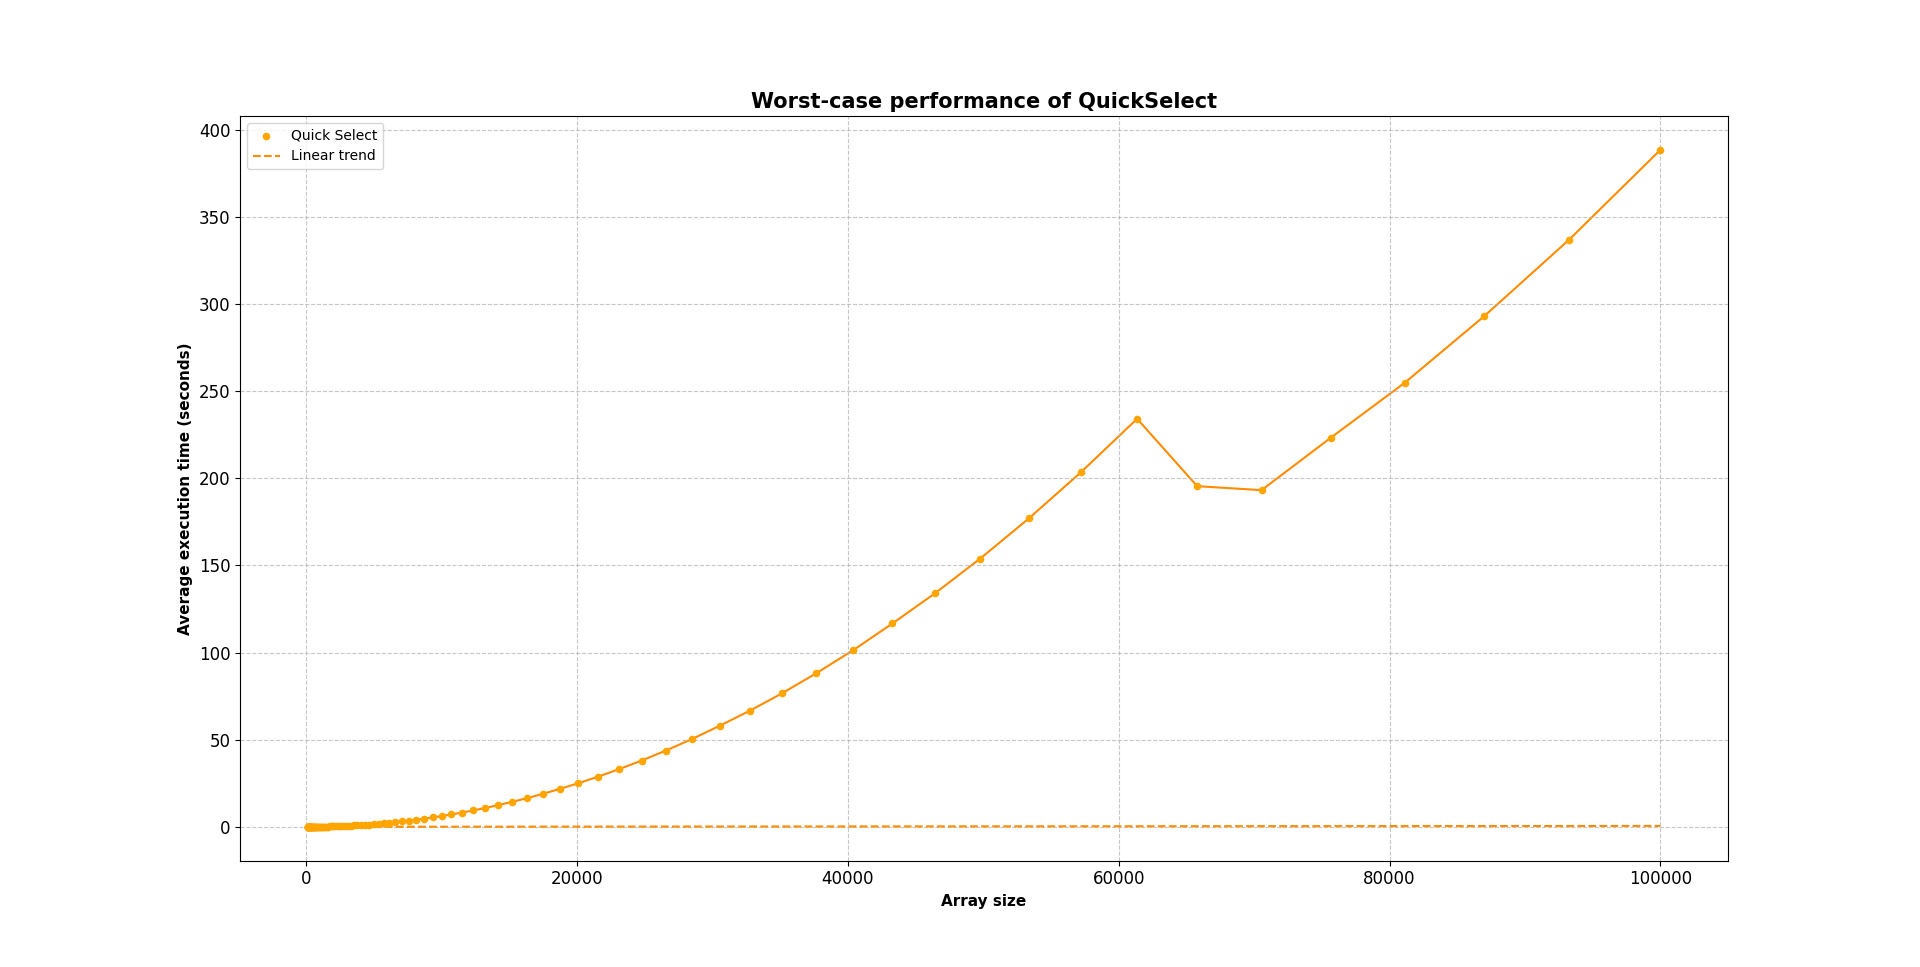
\includegraphics[width=1.2\textwidth]{Graphs/Quick Select/Worst_notLog.png}
  }
  \caption{Worst-case performance of Quick Select - Linear}
\end{figure}

\subsection{Median Of Medians Select}
To improve $QuickSelect$, $partition$ should take as pivot the median of the array at each iteration (element that would be at position $k=len(array)//2$, if the array were ordered).
The idea of $MedianOfMediansSelect$ was based on this very concept.
This algorithm was implemented in an 'almost in place' version in that it did not use auxiliary structures, but made use of recursive calls.
The median was found by the procedure $RecMedianOfMediansSelect$, which performed the following operations:
\begin{enumerate}
    \item Divided the array into blocks of 5 elements and sorted them with $Insertion$ $Sort$
    \item Moved the median of each block to the top of the array
    \item Recursively called itself in the head portion of the array, containing the medians
    \item Moved the median of the medians to the bottom of the array when it came to consider a head sub-array of 5 elements (base case)
    \item Called $Partition$ and called $RecMedianOfMedians$ recursively in the half of the array containing the element sought until the median of the medians was the $k$-$th$ element sought
\end{enumerate}
The $MedianOfMediansSelect$ algorithm has a worst-case complexity of $\Theta(n)$.
In general, we can say that it is the least variable of the three and maintains the same complexity in the average case.\\
Below there are graphs (logarithmic and linear) of the performance of $MedianOf$ $MediansSelect$ in the average case. \\
The dotted line represents the linear performance.\\

\begin{figure}[H]   %MEDIANS OF MEDIANS GRAPH
  \makebox[\textwidth][c]{
    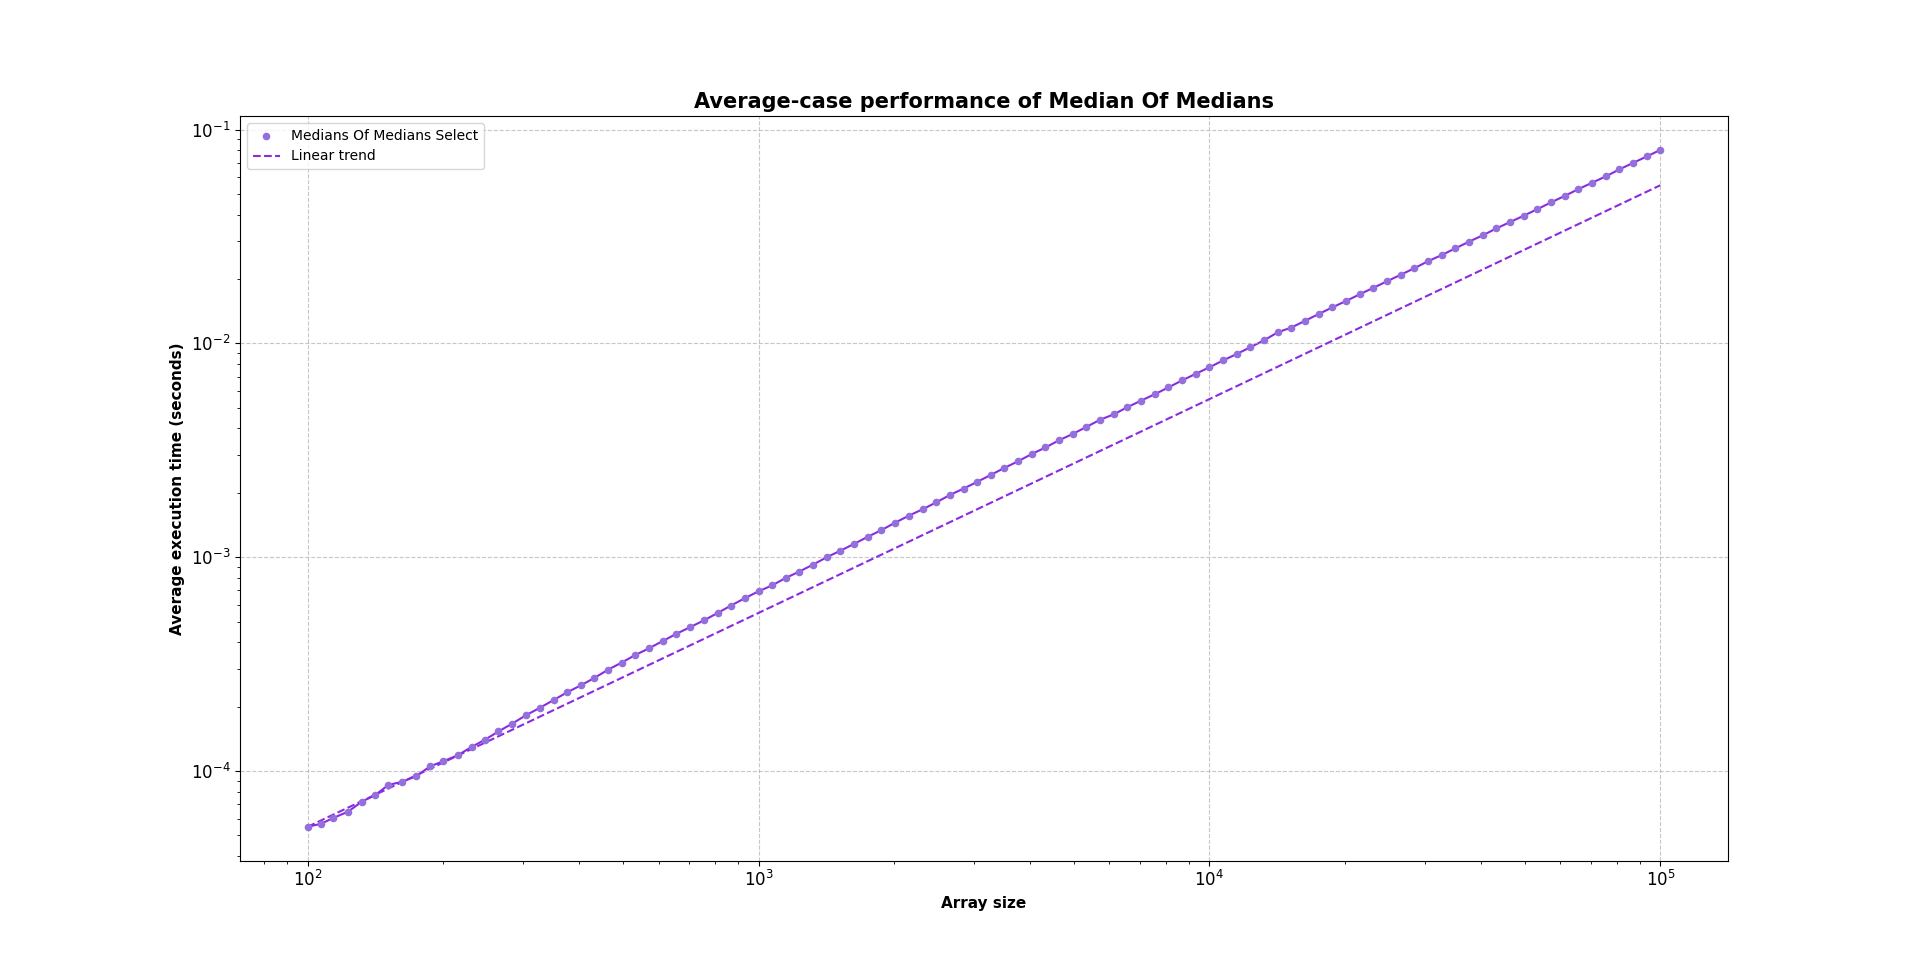
\includegraphics[width=1.2\textwidth]{Graphs/MedianOfMedians Select/kIsRandom_Log.png}
  }
  \caption{Average-case performance of Median Of Medians Select - Logarithmic}
\end{figure}

\begin{figure}[H]   %MEDIANS OF MEDIANS GRAPH
  \makebox[\textwidth][c]{
    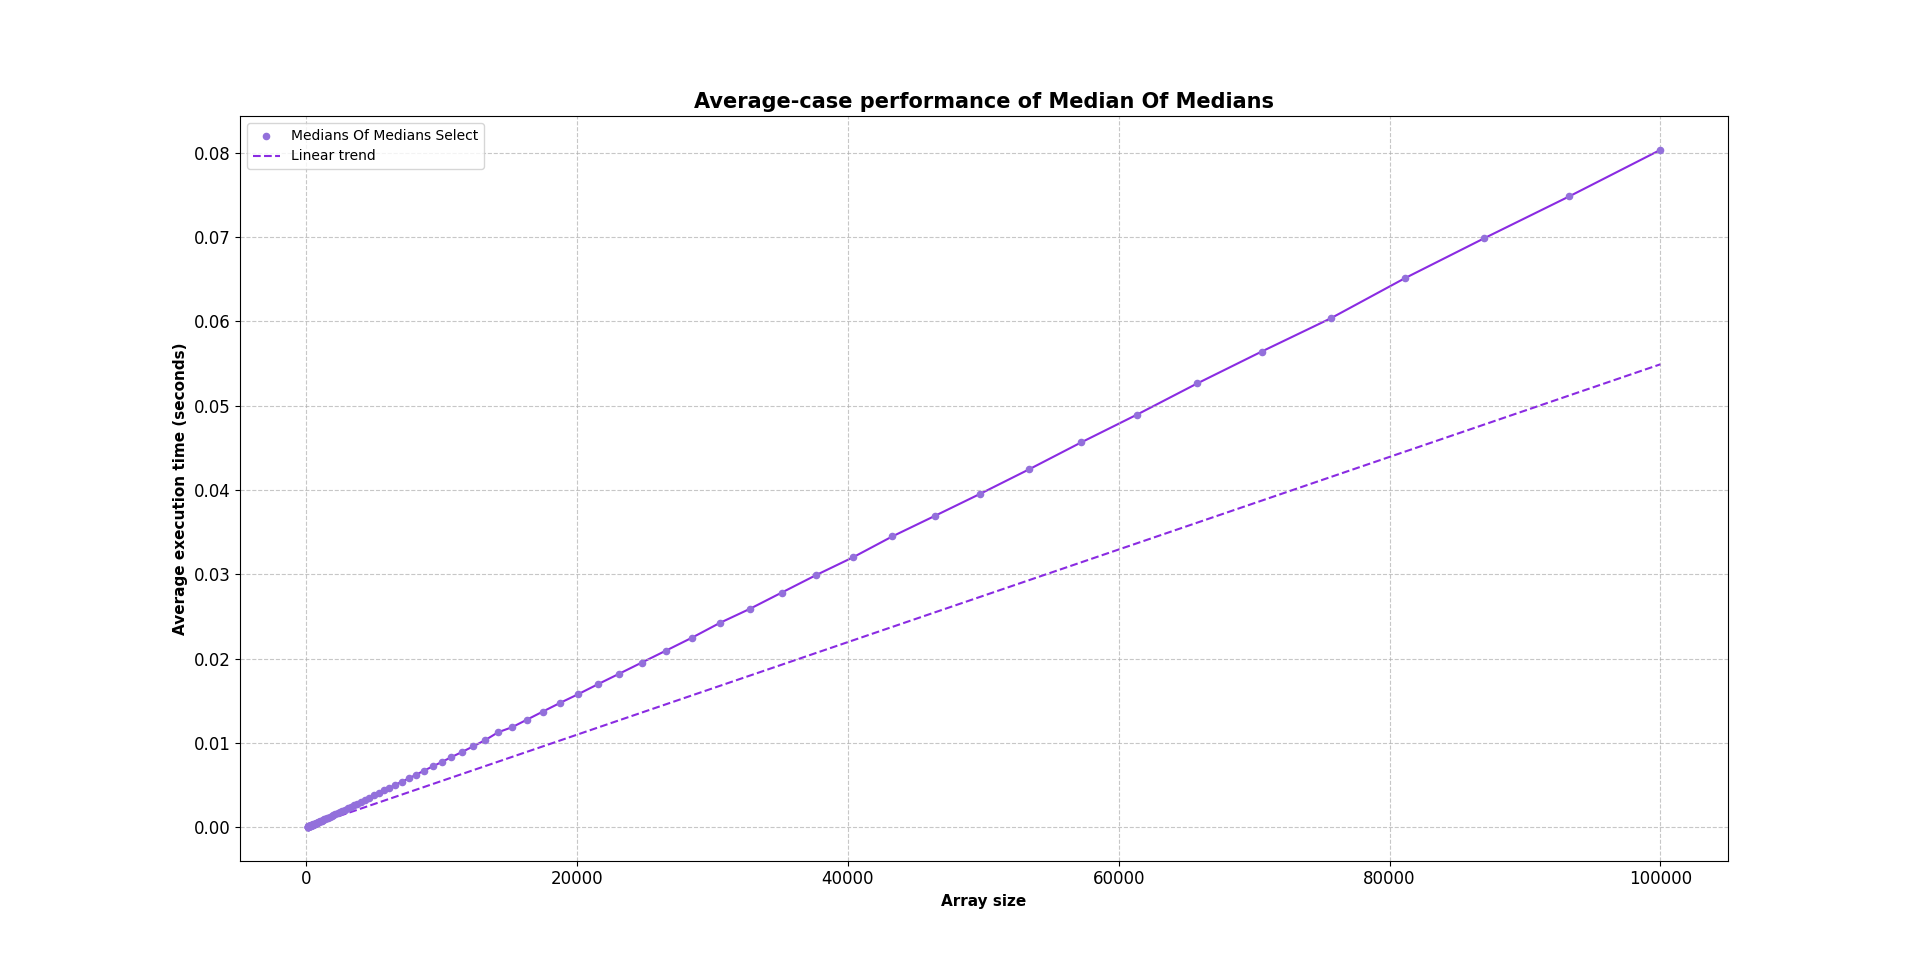
\includegraphics[width=1.2\textwidth]{Graphs/MedianOfMedians Select/kIsRandom_notLog.png}
  }
  \caption{Average-case performance of Median Of Medians Selectn- Linear}
\end{figure}

\subsection{Heap Select}
To find the smallest element in a minHeap, it is sufficient to return its root. Similarly, to find the largest element in a maxHeap it is sufficient to return its root.\\
The algorithm exploited this property to find the $k$-$th$ smallest largest element by extracting $k$-1 times the root.\\
Specifically, after validating the index $k$, if it was less than half the length of the heap, the function constructed a minHeap from H1 and initialized H2 as a minHeap containing a tuple [$element$, $position$] where $element$
corresponded to the root of H1 and $position$ corresponded to the position of that $element$.\\
Otherwise, it constructed a maxHeap from H1 and initialized H2 as a maxHeap of tuples. In the latter case, the problem was reformulated to find the $k$-$th$ largest element, then $k$ was recalculated as $len(H1)-k+1$.\\
After that, the function iterated the following process:
\begin{enumerate}
    \item Extracted the root of H2
    \item Found the left and right children of the extracted position in heap H1
    \item Inserted the children found in H2 (if any)
\end{enumerate}
After iterating $k$-$1$ times, the function returned the root of H2 which corresponded to the $k$-$th$ smallest element. \\
$HeapSelect$ has complexity O$(n+k*log(k))$ in both the worst and average cases. It should, therefore, be preferable to $QuickSelect$ for very small $k$.\\
Below are graphs (logarithmic and linear) of the performance of $HeapSelect$ in the average case. \\
The dotted line represents the linear performance.

\begin{figure}[H]   
  \makebox[\textwidth][c]{%
    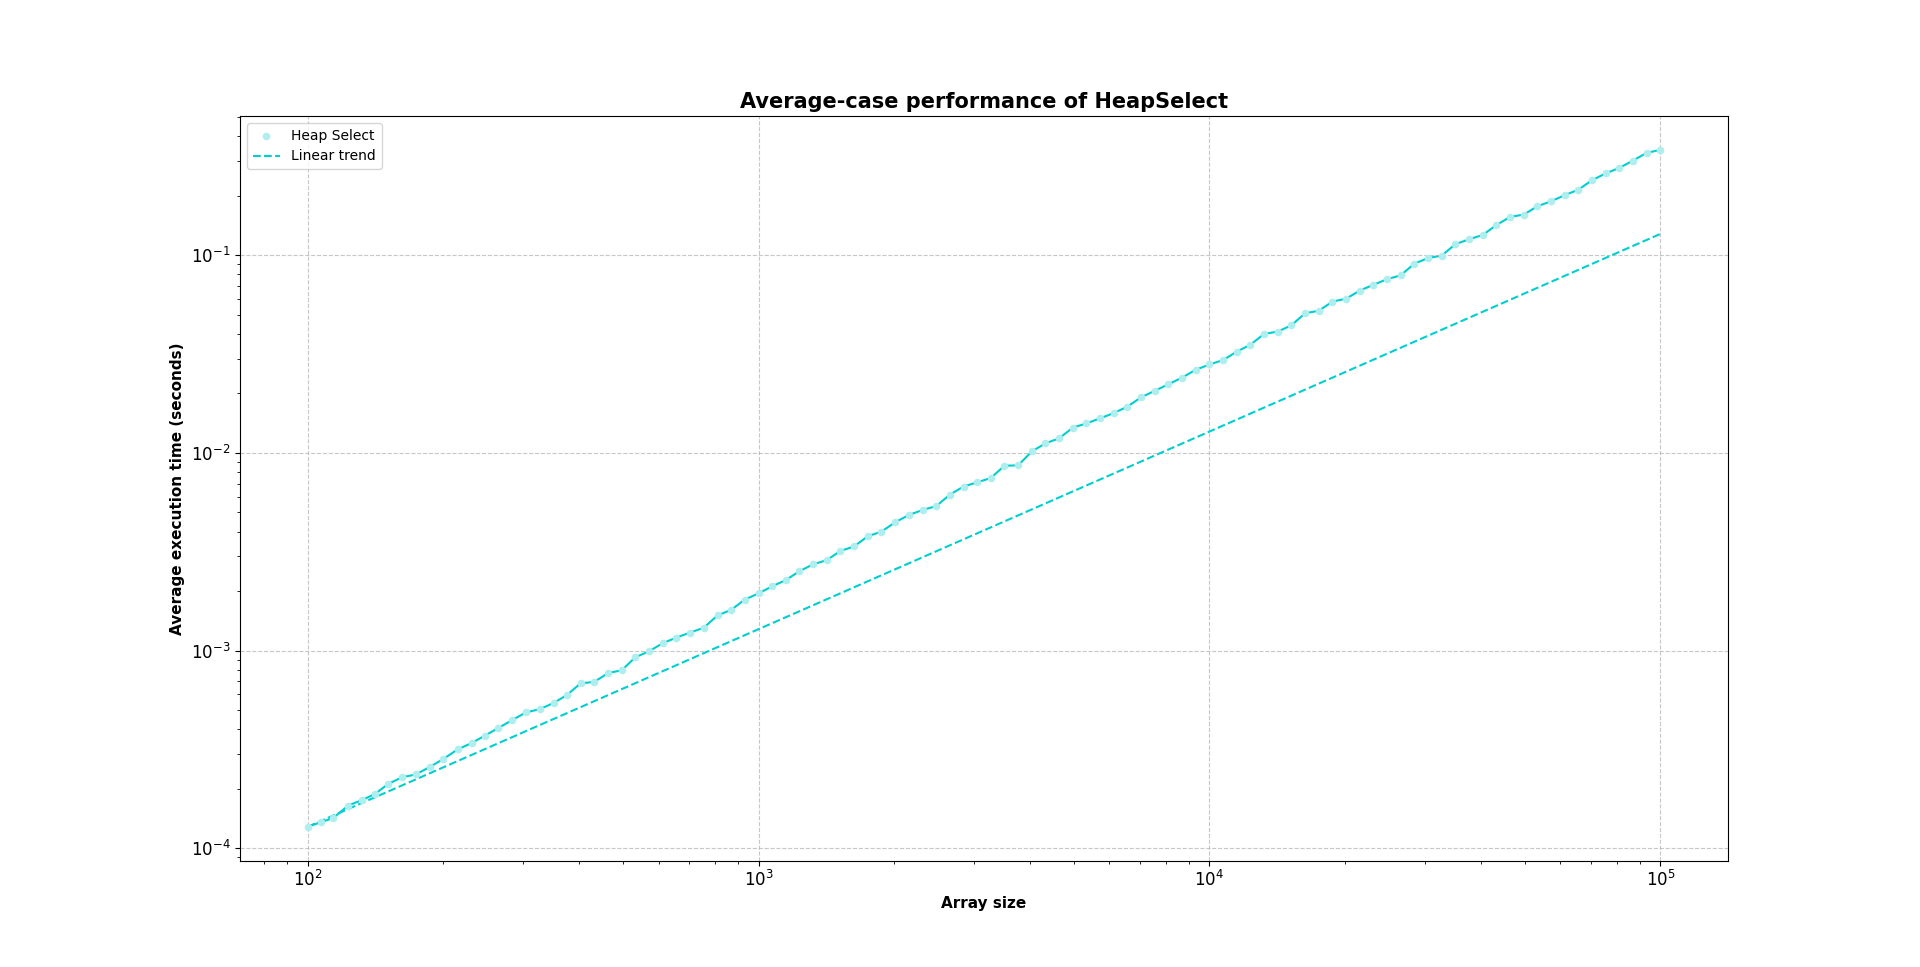
\includegraphics[width=1.2\textwidth]{Graphs/Heap Select/kIsRandom_Log.png}
  }
  \caption{Average-case performance of Heap Select - Logarithmic}
\end{figure} 

\begin{figure}[H]   
  \makebox[\textwidth][c]{%
    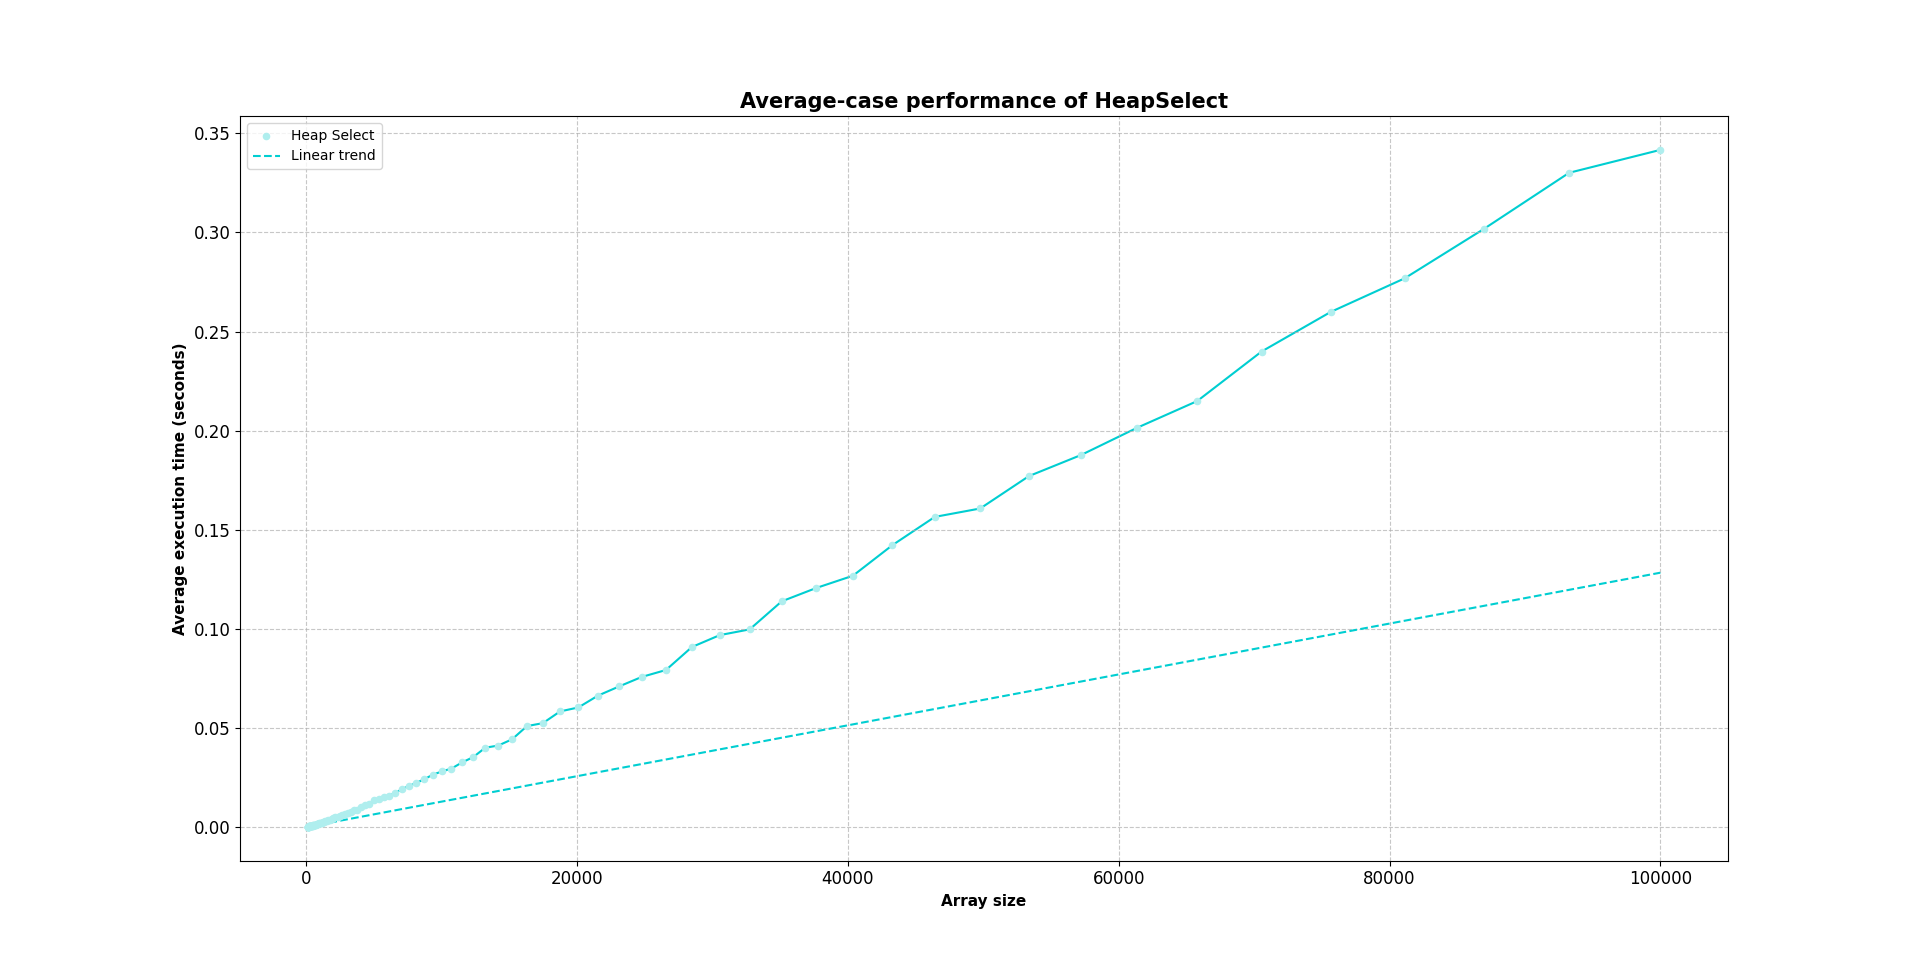
\includegraphics[width=1.2\textwidth]{Graphs/Heap Select/kIsRandom_notLog.png}
  }
  \caption{Average-case performance of Heap Select - Linear}
\end{figure} 

\section{Benchmark}
The $benchmark$ measured the average execution time of each algorithm in the $algorithmOfSuccession$ array.\\
It generated 100 ($stepSuccession$) arrays of increasing size following a geometric series. The size of the arrays ranged from 100 to 100000.\\
For each sort algorithm, for each array:
\begin{enumerate} %Enumerated list starts
    \item 500 ($testPerEachN$) tests were run with random $k$, to make it possible to calculate the average time for each algorithm. At each test: 
    \begin{itemize} %Dotted list starts
        \item The array was filled with random values in the range [-1000, 1000]
        \item The execution time was measured (for each of the algorithms) to ensure a relative error of less than 1\%
        \item Average execution times were saved in a matrix ($averagetimes$)
    \end{itemize} %Dotted list ends
    
    \item In a matrix ($timesAverage$), there were stored:
    \begin{itemize} %Dotted list starts
        \item The size of the array considered
        \item The average execution time
    \end{itemize} %Dotted list ends
    
\end{enumerate} %Enumerated list ends
At the end of the 100 ($stepSuccession$) steps, the average times were saved in separate files, one for each algorithm.
Finally, the function that drew the graph was called, and it used the values from the generated files to draw said graphs.

\section{Experiments}
\subsection{K Dependence}
To evaluate the dependence on the chosen parameter $k$, we performed four further tests:
\begin{enumerate}
    \item Fixed array size at 1000 and $k=0,10,20,...,1000$
    \item Variable array size and $k=1$
    \item Variable array size and $k=len(array)//2$
    \item Variable array size and $k=len(array)$
\end{enumerate}
1. In the first test, we obtained the following graph from which the $k$ dependence of $HeapSelect$ was particularly evident: \\

\begin{figure}[H]   
  \makebox[\textwidth][c]{%
    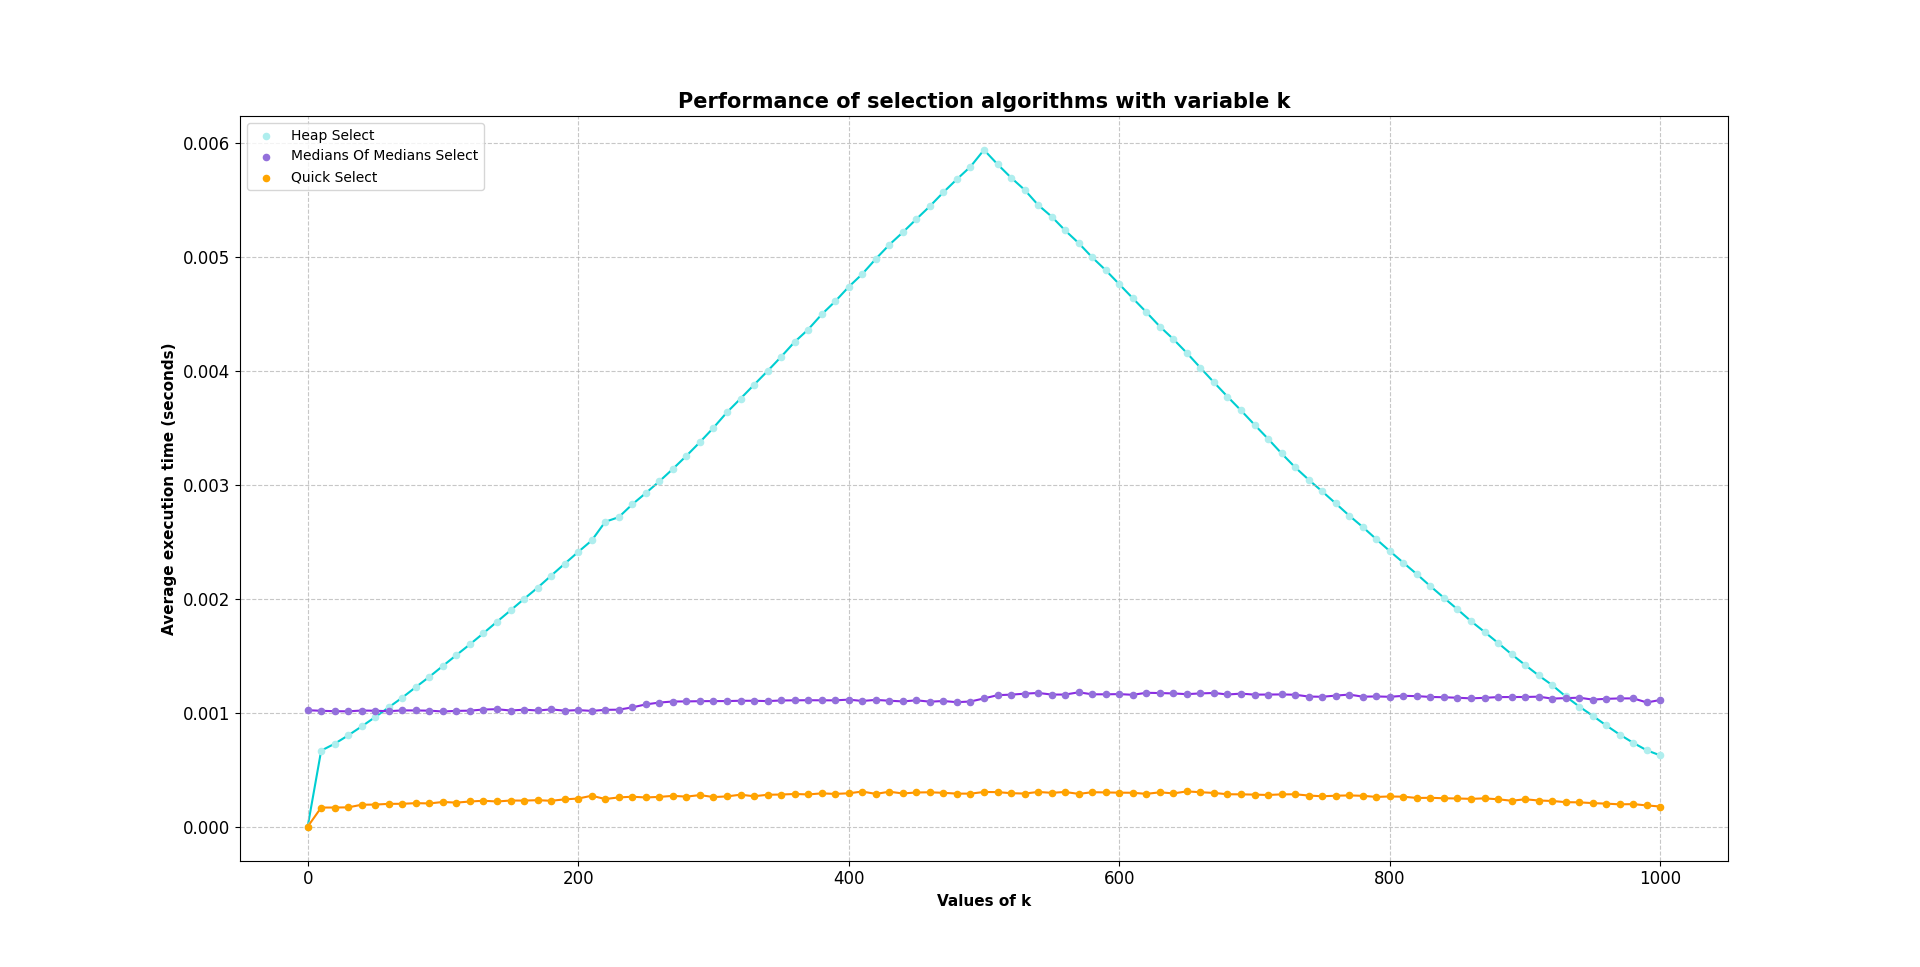
\includegraphics[width=1.2\textwidth]{Graphs/K Variations/kIs10x.png}
  }
  \caption{k=0,10,20,...,1000}
\end{figure} 


2. For $k=1$ we fell into the best possible case for $HeapSelect$, which was super linear and less variable than its average case with random $k$.\\

\begin{figure}[H]   
  \makebox[\textwidth][c]{%
    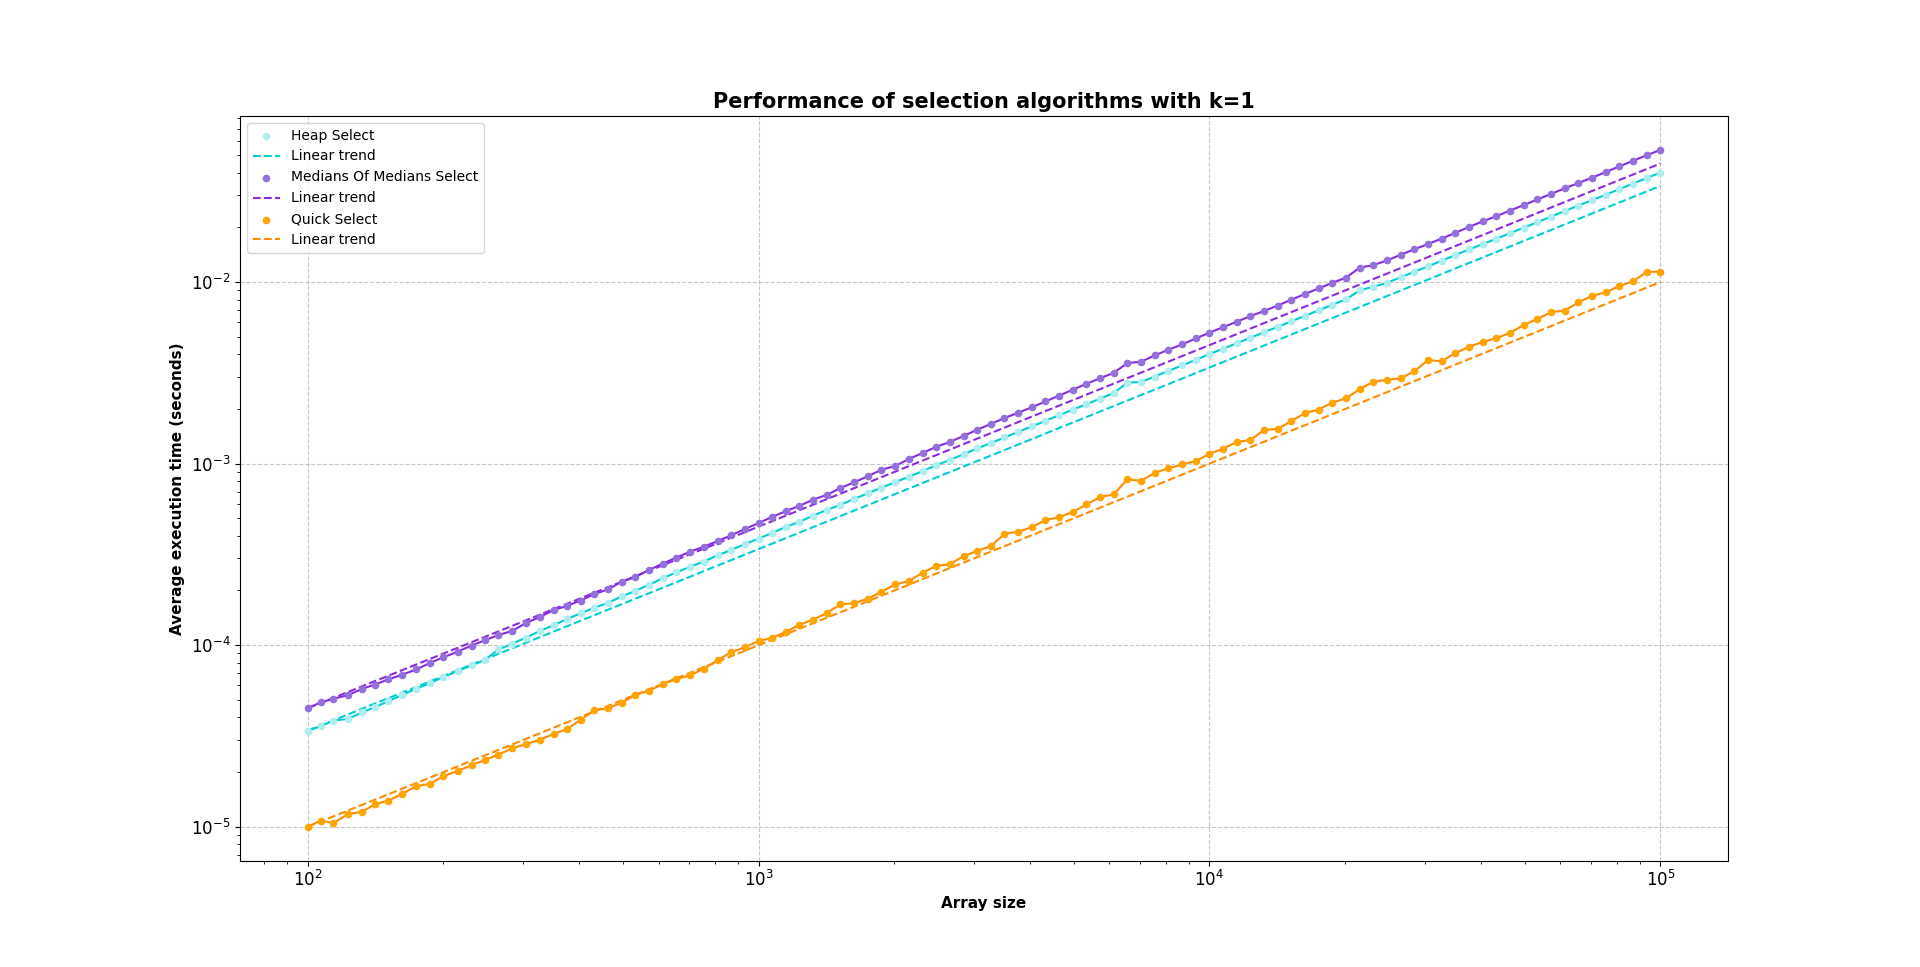
\includegraphics[width=1.2\textwidth]{Graphs/K Variations/kIs1_Log.png}
  }
  \caption{Performance of selection algorithms for k=1 - Logarithmic}
\end{figure}
\begin{figure}[H]   
  \makebox[\textwidth][c]{%
    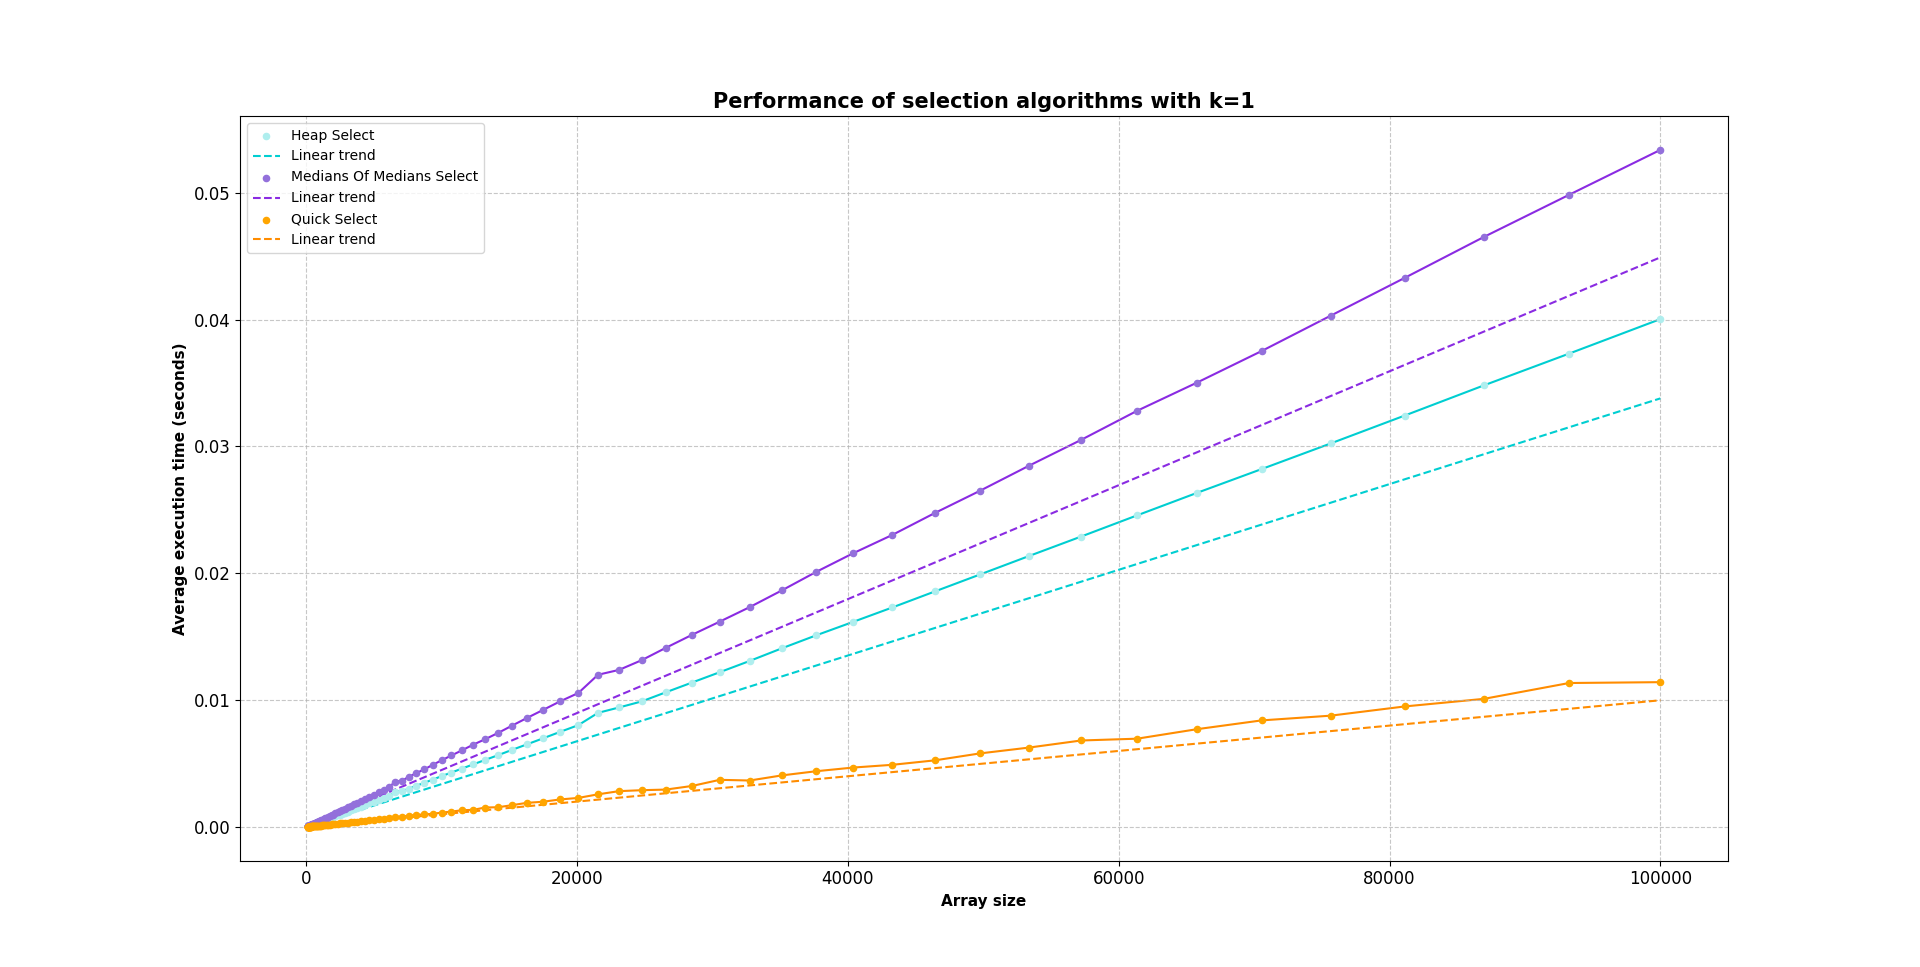
\includegraphics[width=1.2\textwidth]{Graphs/K Variations/kIs1_notLog.png}
  }
  \caption{Performance of selection algorithms for k=1 - Linear}
\end{figure}

3. For $k=len(array)//2$ we fell into the worst case for $HeapSelect$. In fact, the execution times were higher, the trend remained very similar to that of its average case with random $k$.\\
For $QuickSelect$ and for $MedianOfMediansSelect$ on the other hand, the graph was unchanged.\\

\begin{figure}[H]   
  \makebox[\textwidth][c]{%
    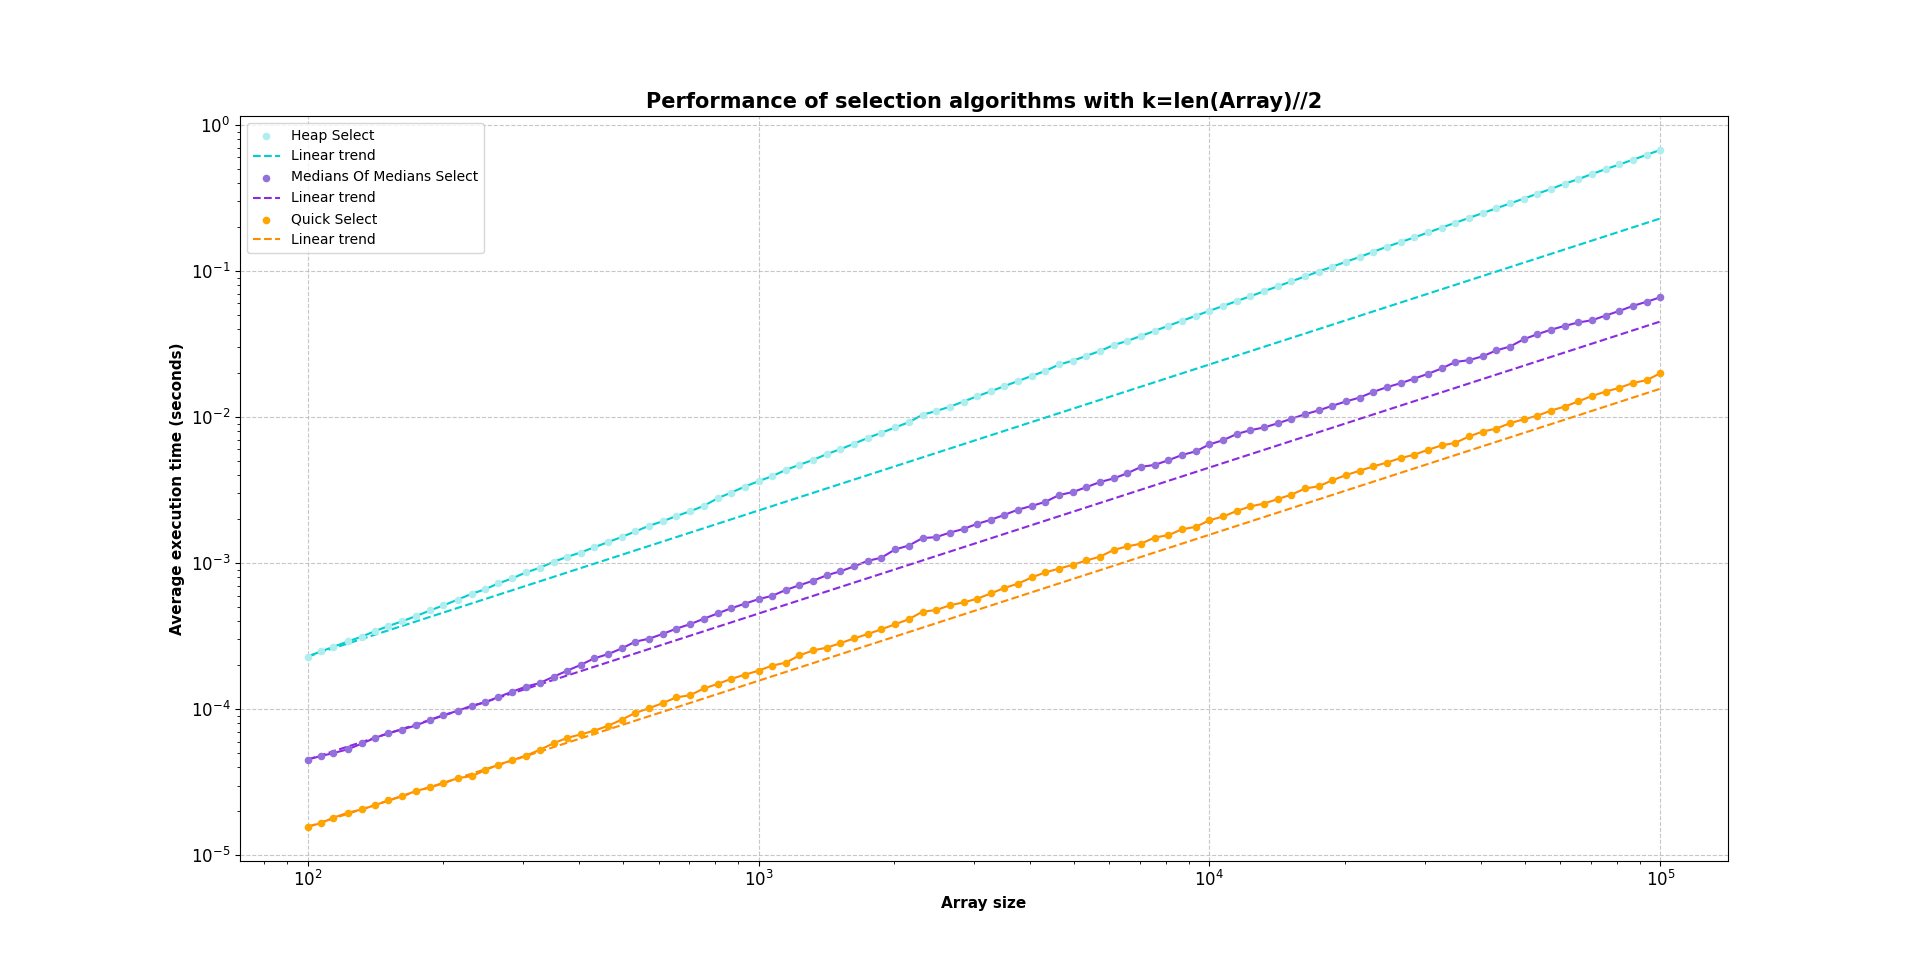
\includegraphics[width=1.2\textwidth]{Graphs/K Variations/kIsLenArrayDiv2_Log.png}
  }
  \caption{Performance of selection algorithms for k=len(array)//2 -Logarithmic}
\end{figure}

\begin{figure}[H]   
  \makebox[\textwidth][c]{%
    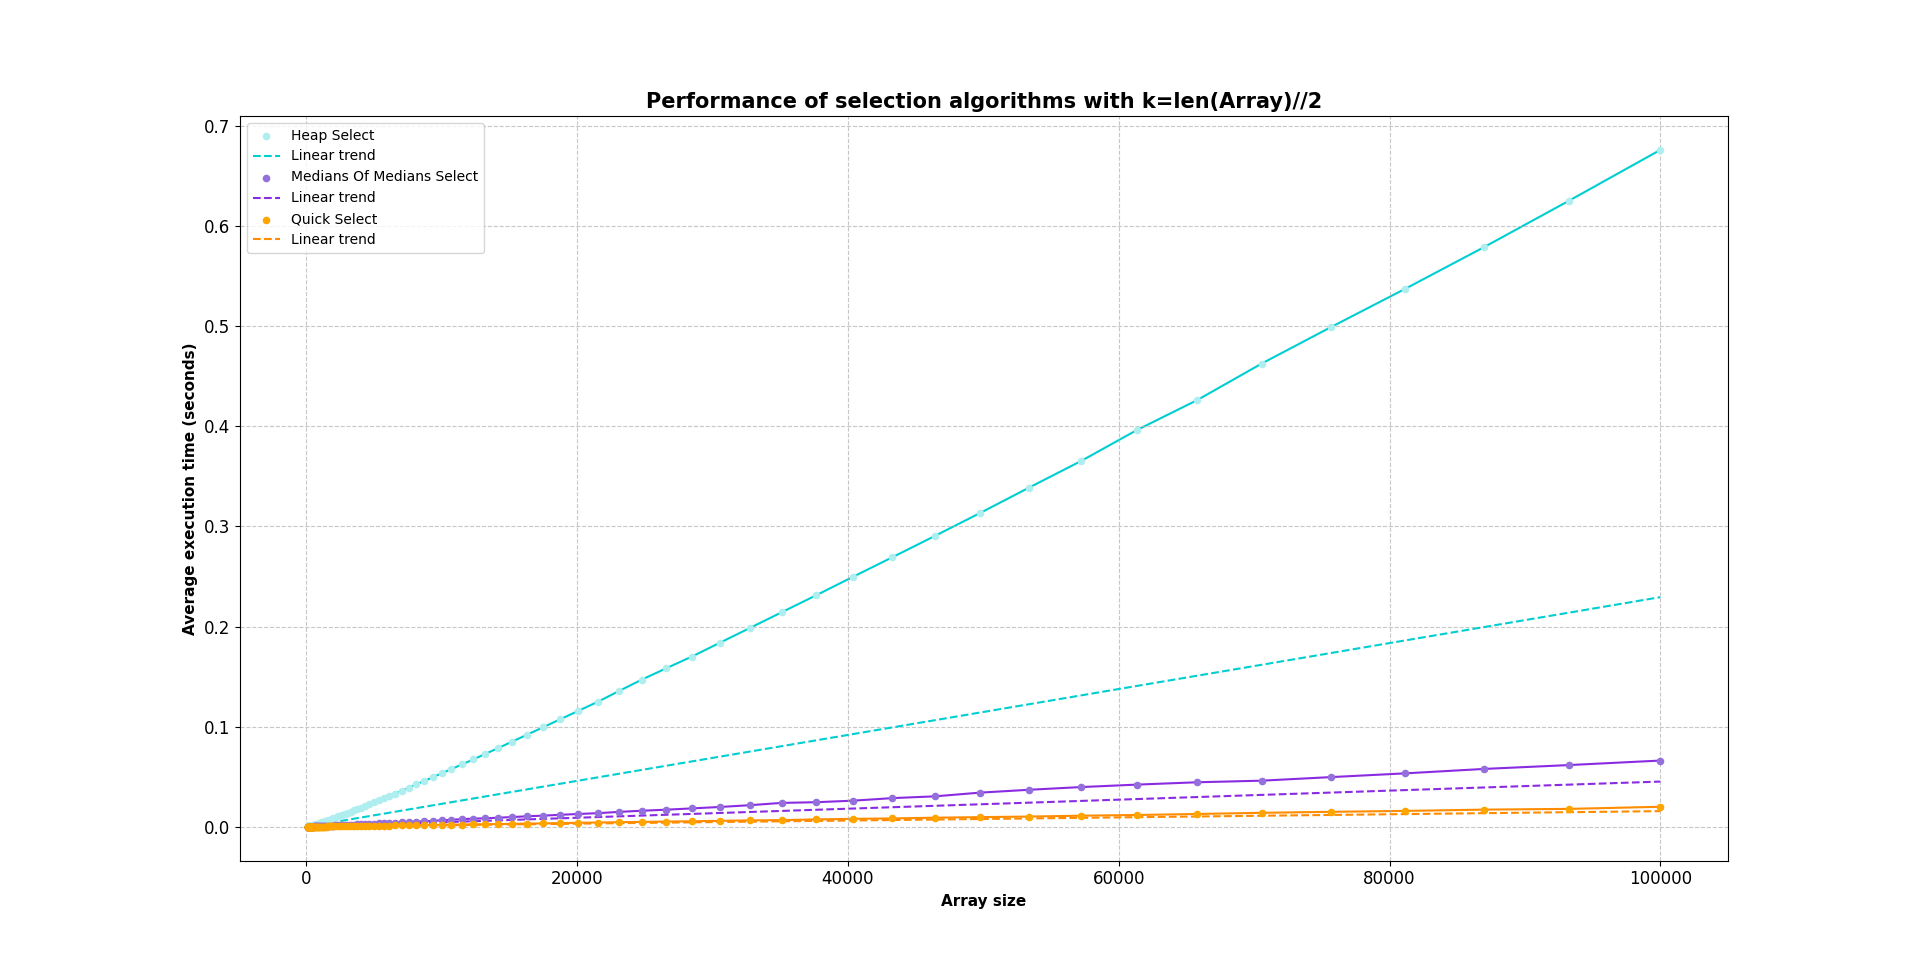
\includegraphics[width=1.2\textwidth]{Graphs/K Variations/kIsLenArrayDiv2_notLog.png}
  }
  \caption{Performance of selection algorithms for k=len(array)//2 - Linear}
\end{figure}

4. For $k=len(array)$ we obtained an analogous case to $k=1$,with the best case for $HeapSelect$.\\

\begin{figure}[H]   
  \makebox[\textwidth][c]{%
    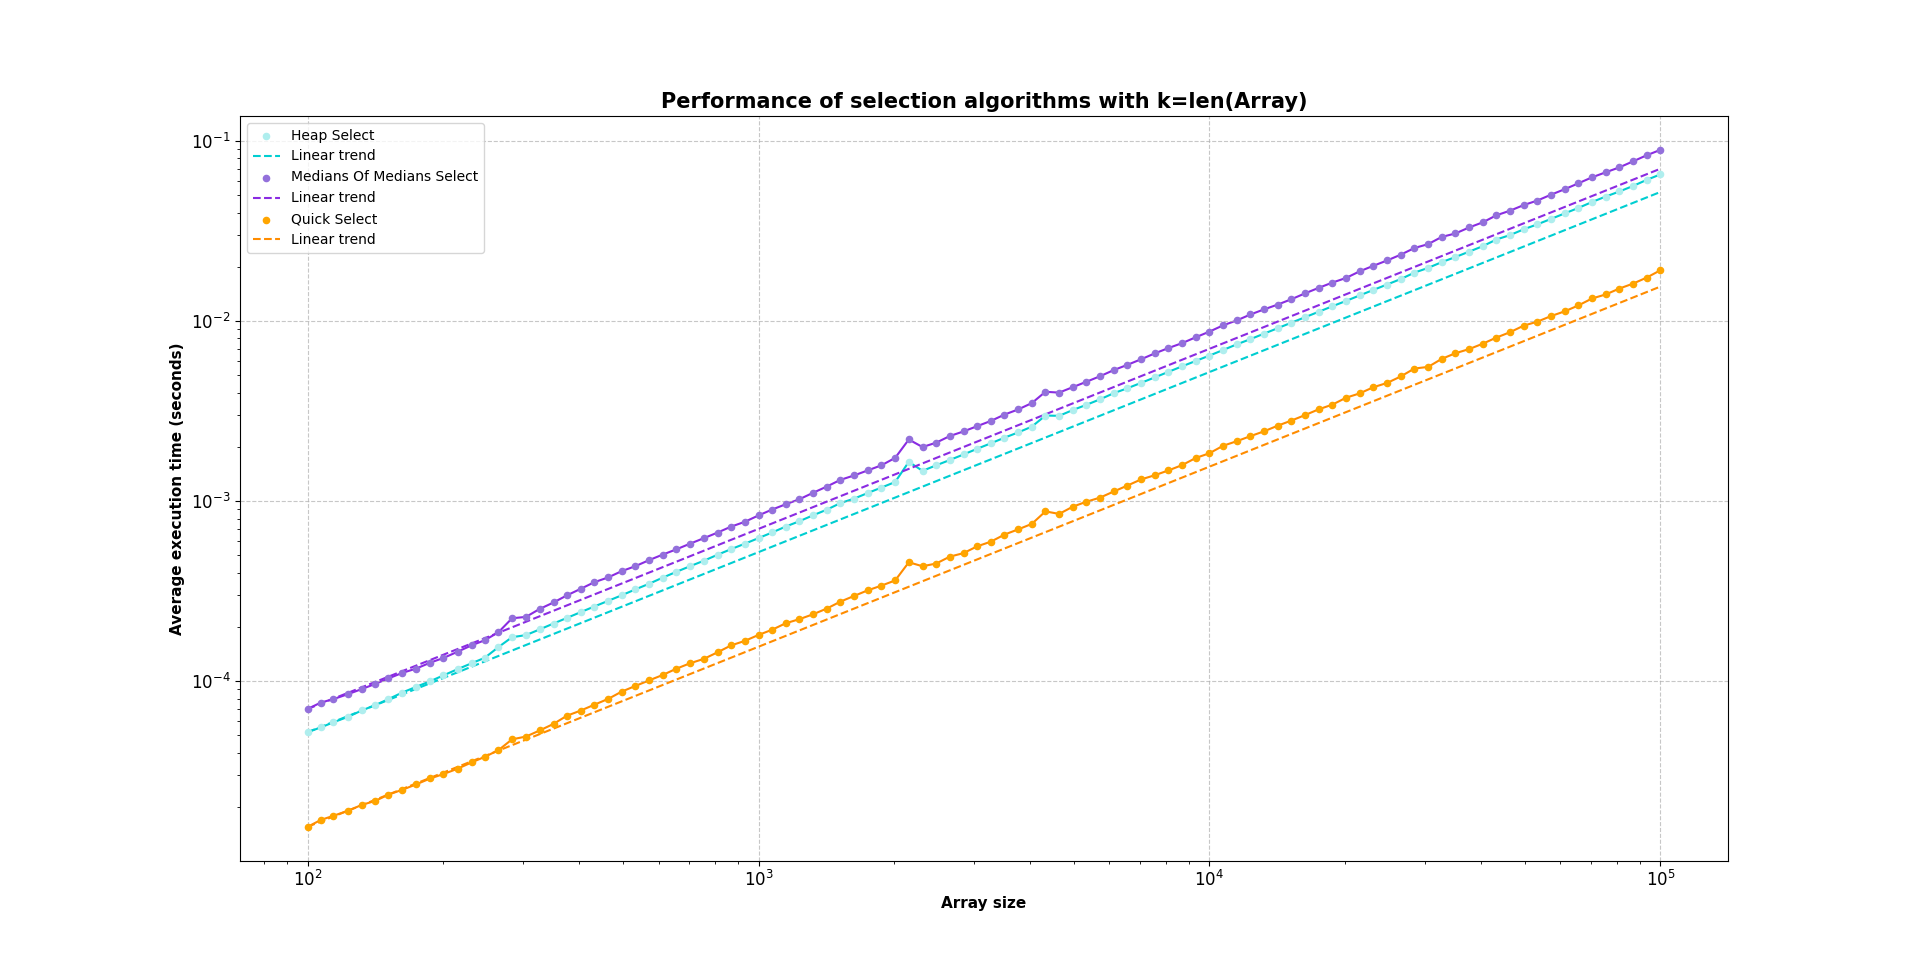
\includegraphics[width=1.2\textwidth]{Graphs/K Variations/kIsLenArray_Log.png}
  }
  \caption{Performance of selection algorithms for k=len(array) - Logarithmic}
\end{figure}

\begin{figure}[H]   
  \makebox[\textwidth][c]{%
    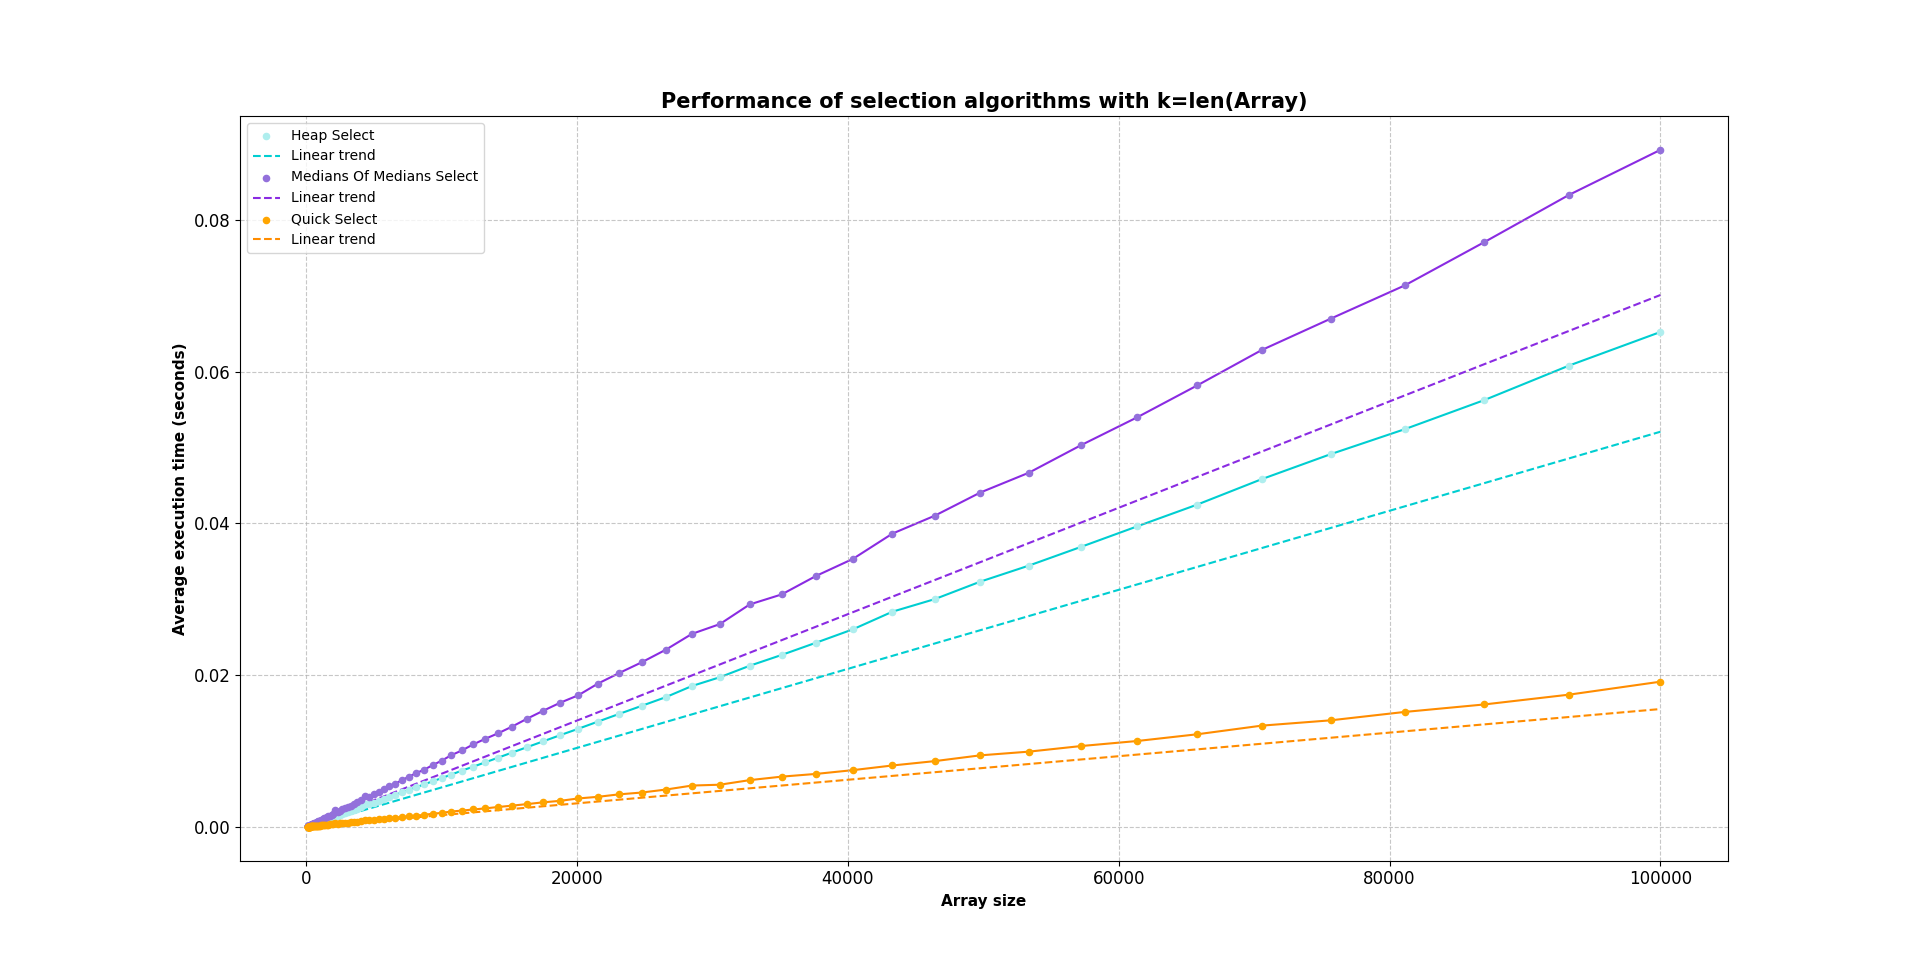
\includegraphics[width=1.2\textwidth]{Graphs/K Variations/kIsLenArray_notLog.png}
  }
  \caption{Performance of selection algorithms for k=len(array) - Linear}
\end{figure}

\subsection{Quick Select using Partition3WayRandomized}
We then wanted to try to improve the complexity of $QuickSelect$ by using $Partition3WayRandomized$ and simulating the same worst-case conditions for $QuickSelect$ (with normal partition), i.e. using arrays sorted in ascending direction and $k=1$, to show that in that case, this version was much more efficient.\\
This test, like all the others, with the exception of the worst-case $QuickSelect$ test, was performed with 500 $testPerOneN$. \\
It is important to emphasize that the proposed conditions did not represent the worst case for this $QuickSelect$. In fact, its worst case is impossible to determine since the pivots of $Partition3WayRandomized$ are chosen randomly.\\

\begin{figure}[H]   
  \makebox[\textwidth][c]{%
    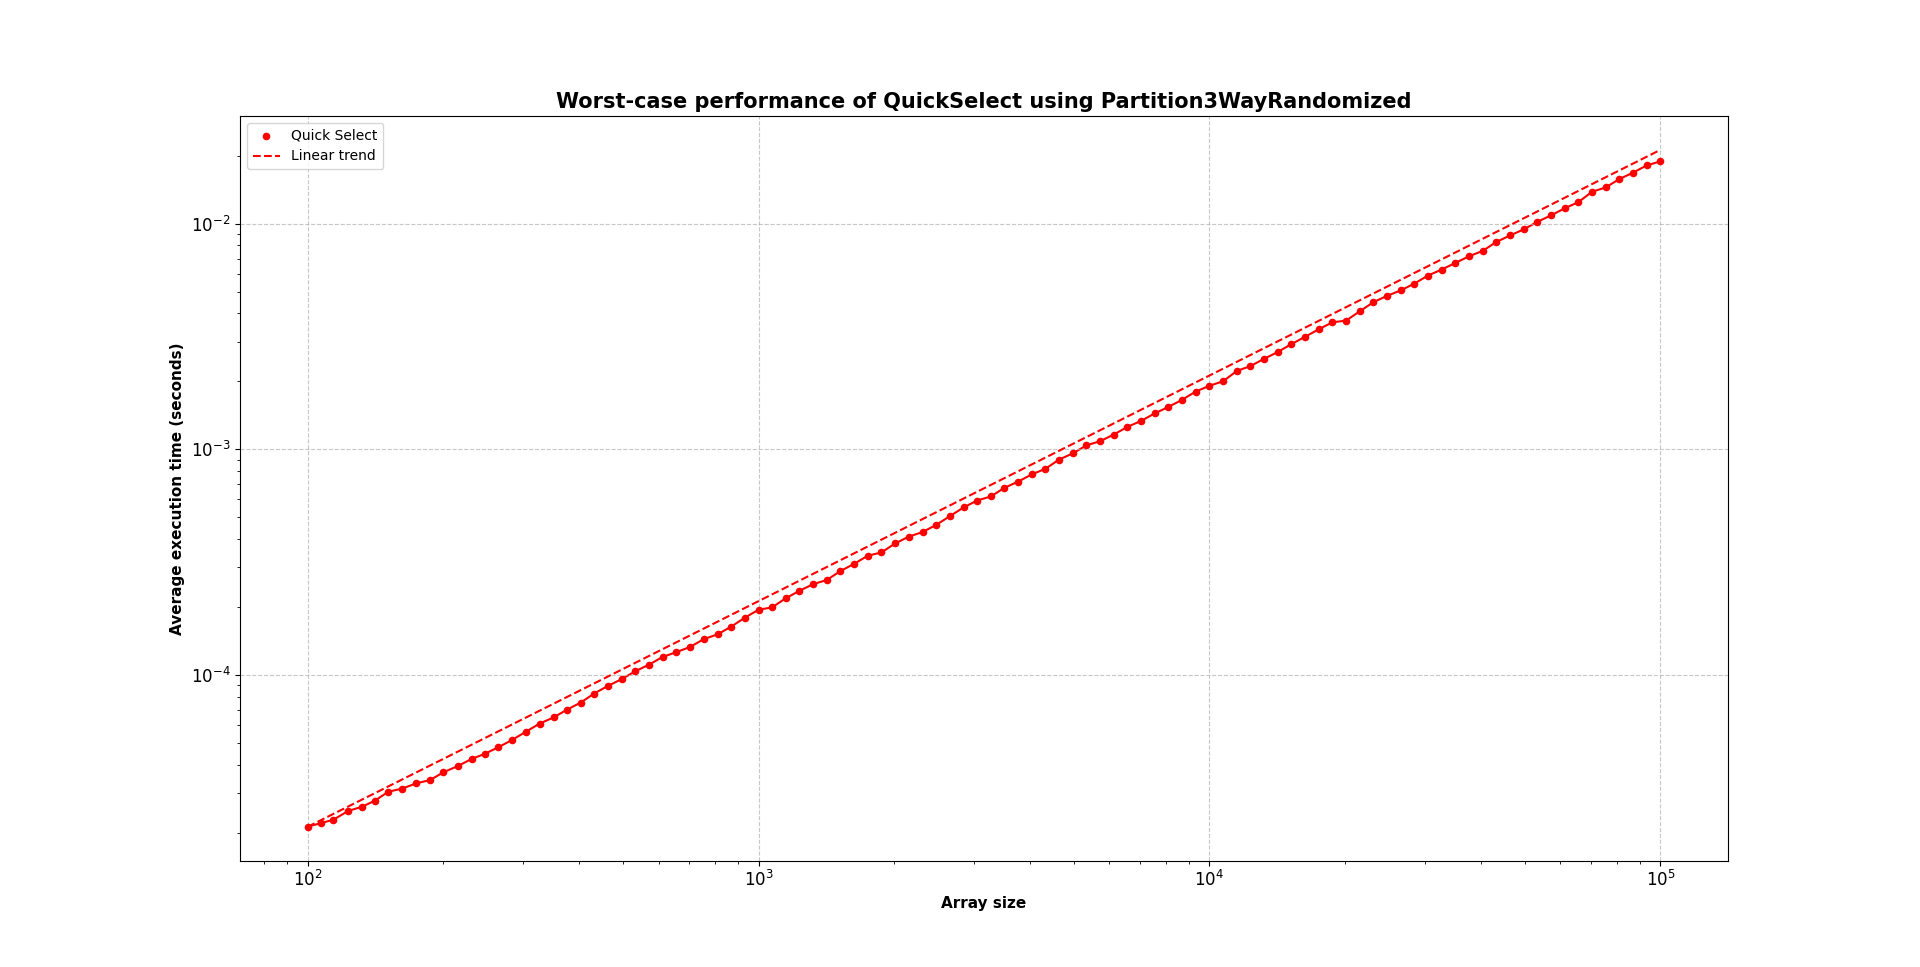
\includegraphics[width=1.2\textwidth]{Graphs/Quick Select P3W/kIsRandom_Log.png}
  }
  \caption{Worst-case performance of Quick Select using Partition3WayRandomized - Logarithmic}
\end{figure}
\begin{figure}[H]   
  \makebox[\textwidth][c]{%
    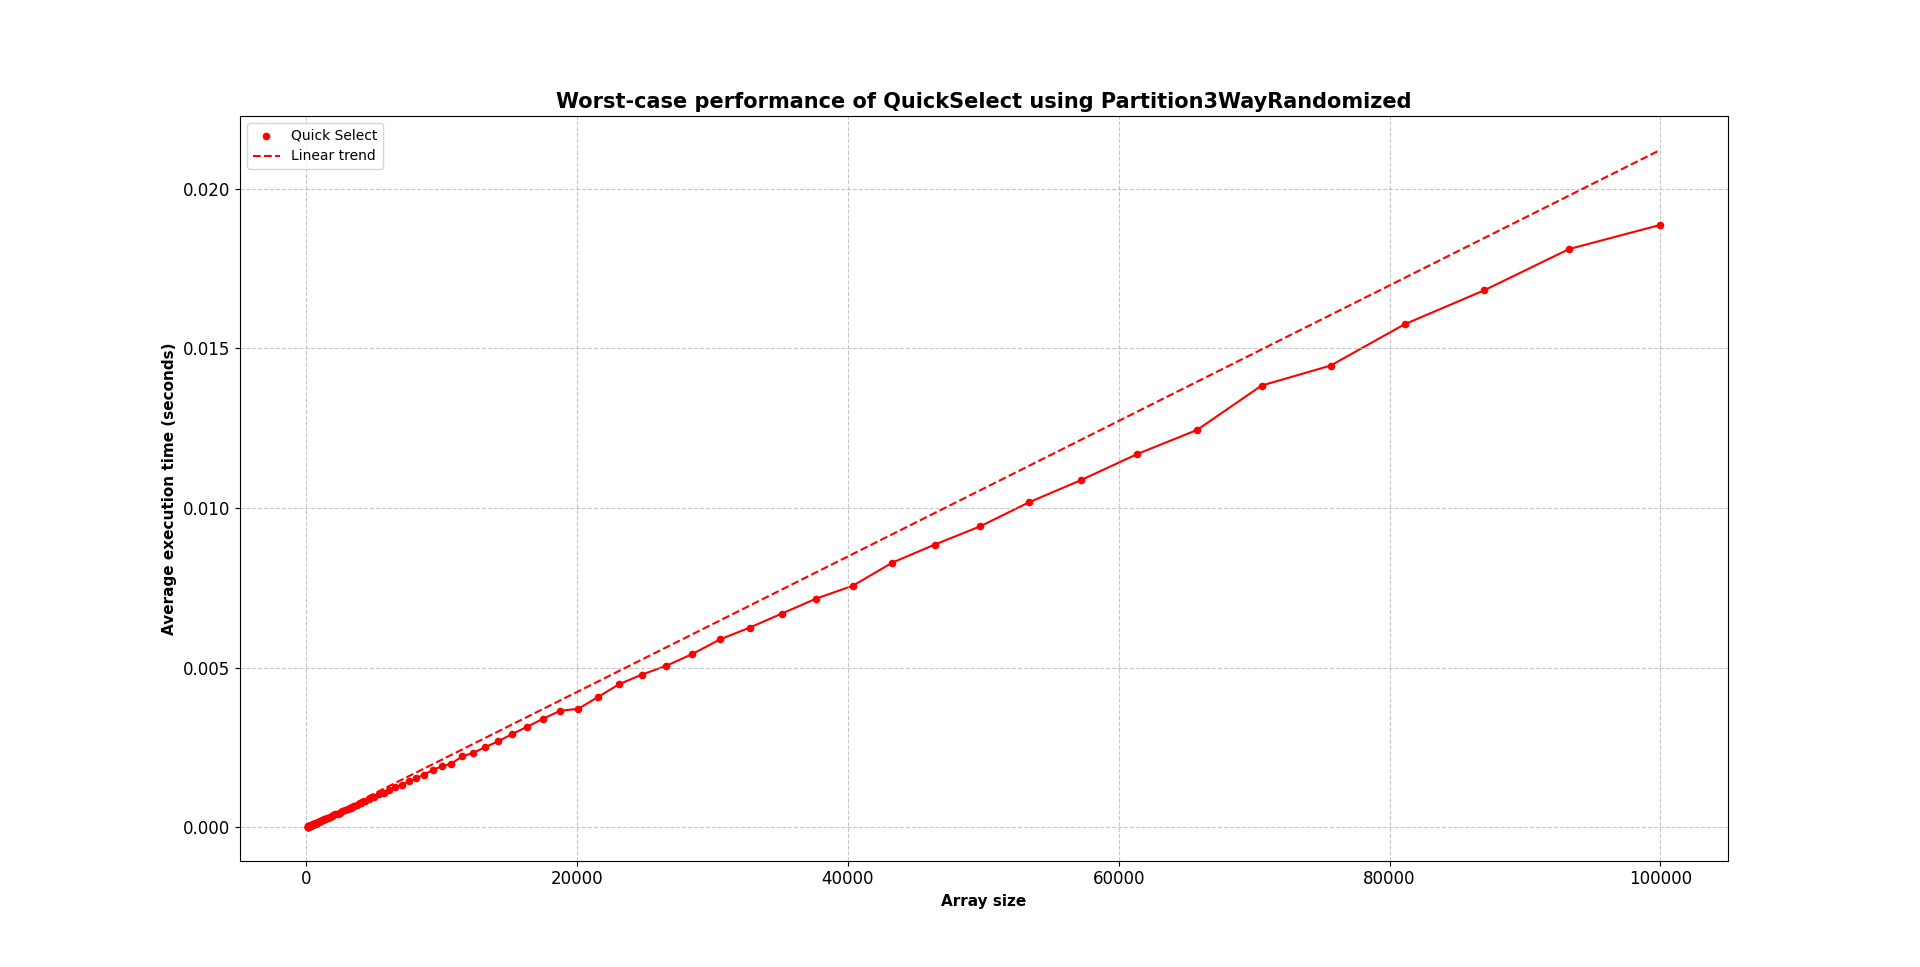
\includegraphics[width=1.2\textwidth]{Graphs/Quick Select P3W/kIsRandom_notLog.png}
  }
  \caption{Worst-case performance of Quick Select using Partition3WayRandomized - Linear}
\end{figure}


\section{Conclusions and final graph}
If we look only at the complexities of the three proposed algorithms, one might think that $QuickSelect$ is the worst of the three. As worst case it has a complexity of $\Theta(n^2)$.\\ However, from the graph it is interesting to note that for random arrays and $k$ the most efficient algorithm was indeed $QuickSelect$, followed by $MedianOfMe$-$dians$ $Select$ and, at the end, $HeapSelect$.

\begin{figure}[H]   
  \makebox[\textwidth][c]{%
    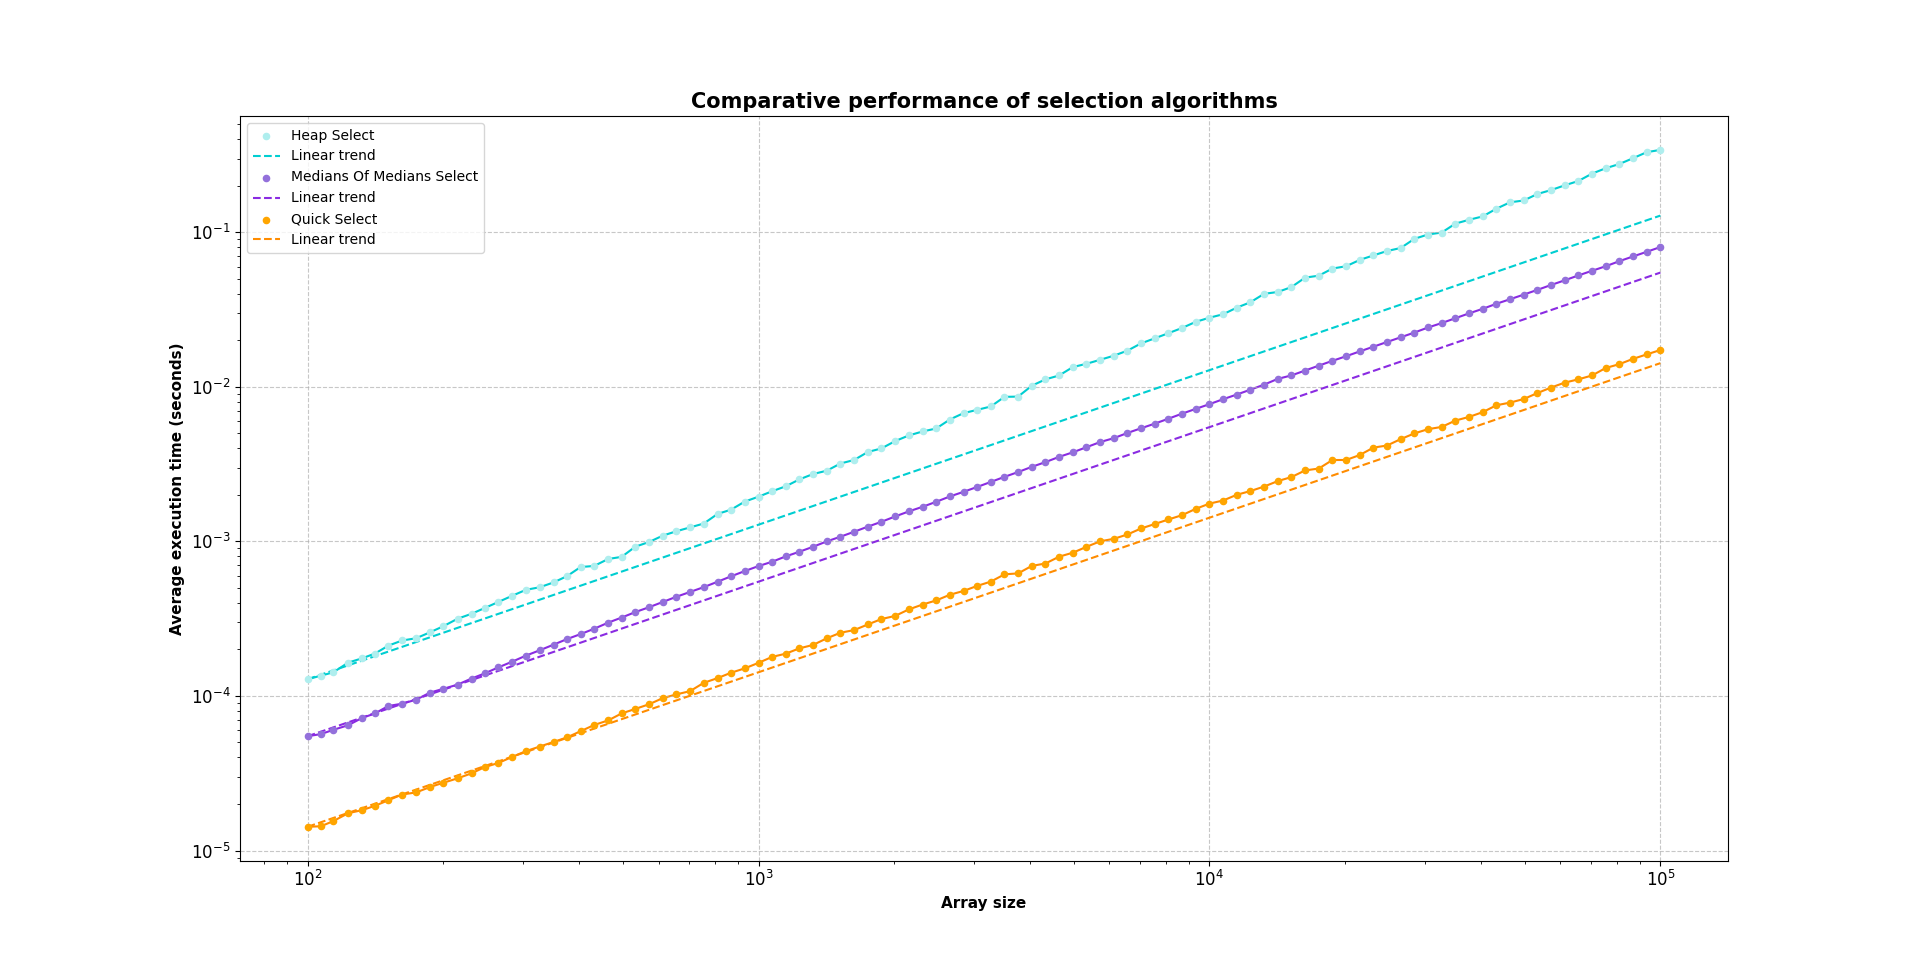
\includegraphics[width=1.2\textwidth]{Graphs/Final Graphs/kIsRandom_Log.png}
  }
  \caption{Comparative performance of selection algorithms - Logarithmic}
\end{figure}

\begin{figure}[H]   
  \makebox[\textwidth][c]{%
    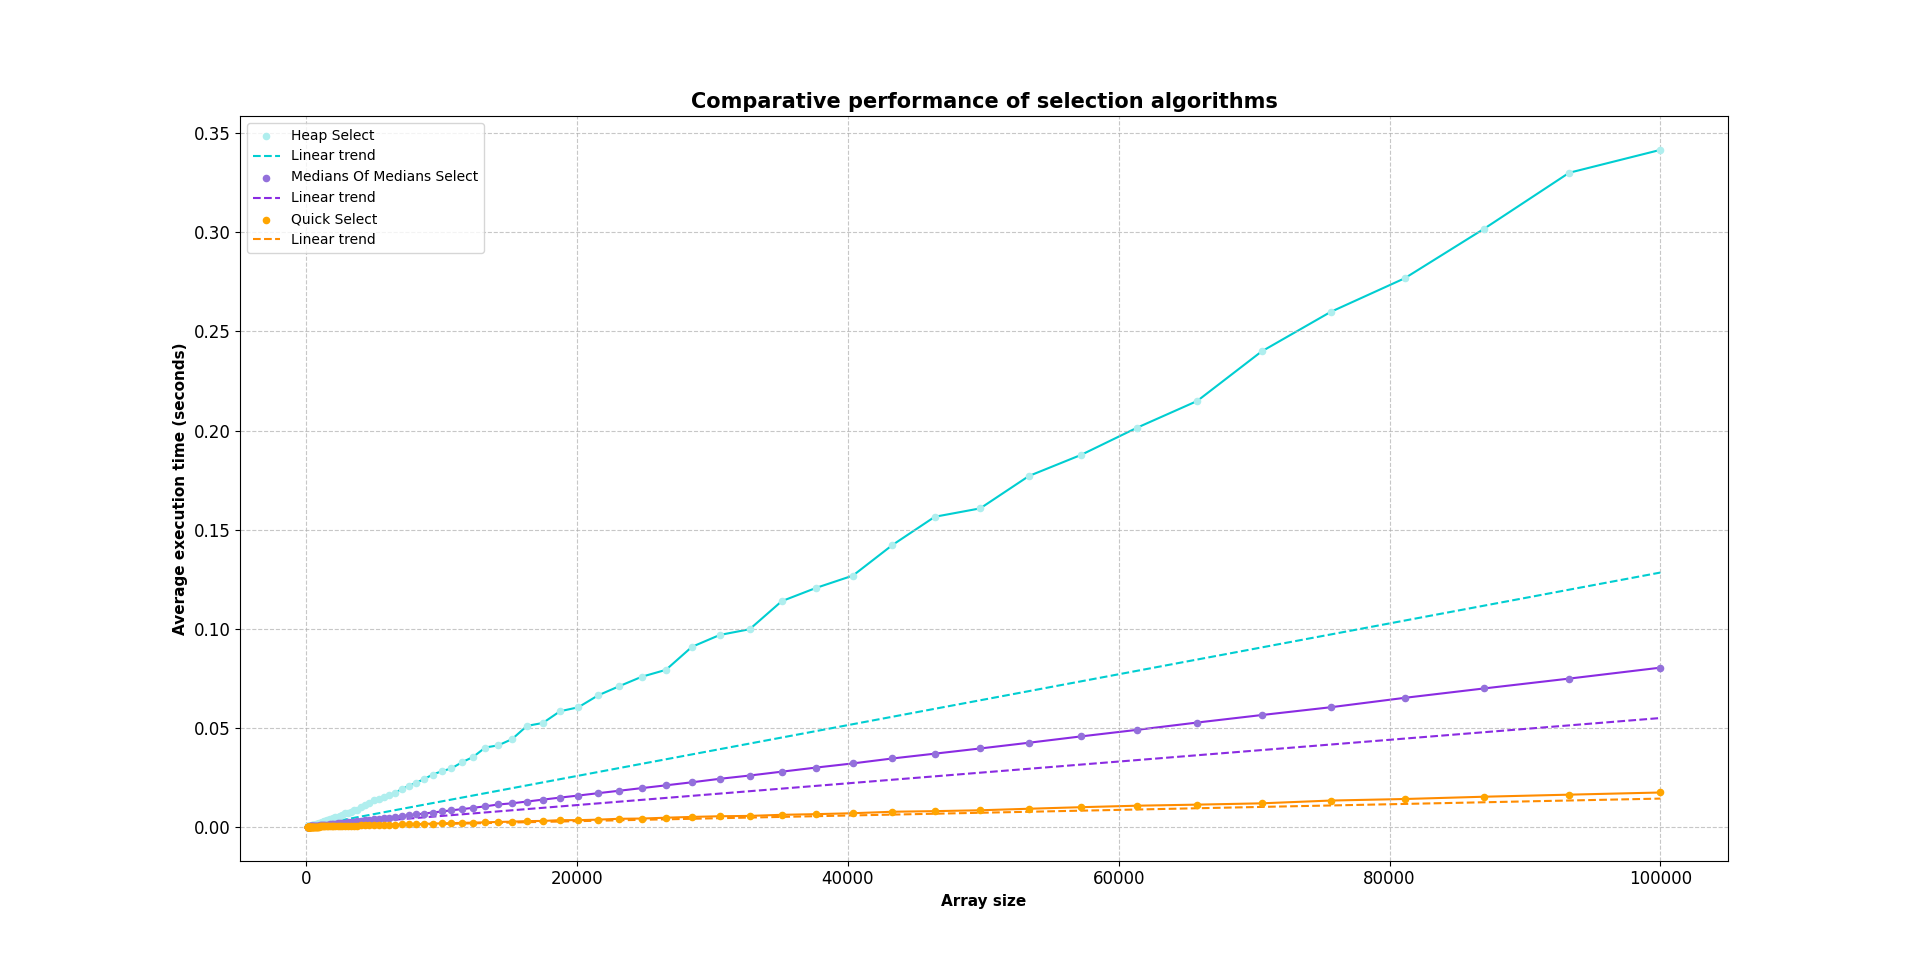
\includegraphics[width=1.2\textwidth]{Graphs/Final Graphs/kIsRandom_notLog.png}
  }
  \caption{Comparative performance of selection algorithms - Linear}
\end{figure}

Using $QuickSelectRandomized$ with $Partition3WayRandomized$ in the average case we obtained the following graphs:

\begin{figure}[H]   
  \makebox[\textwidth][c]{%
    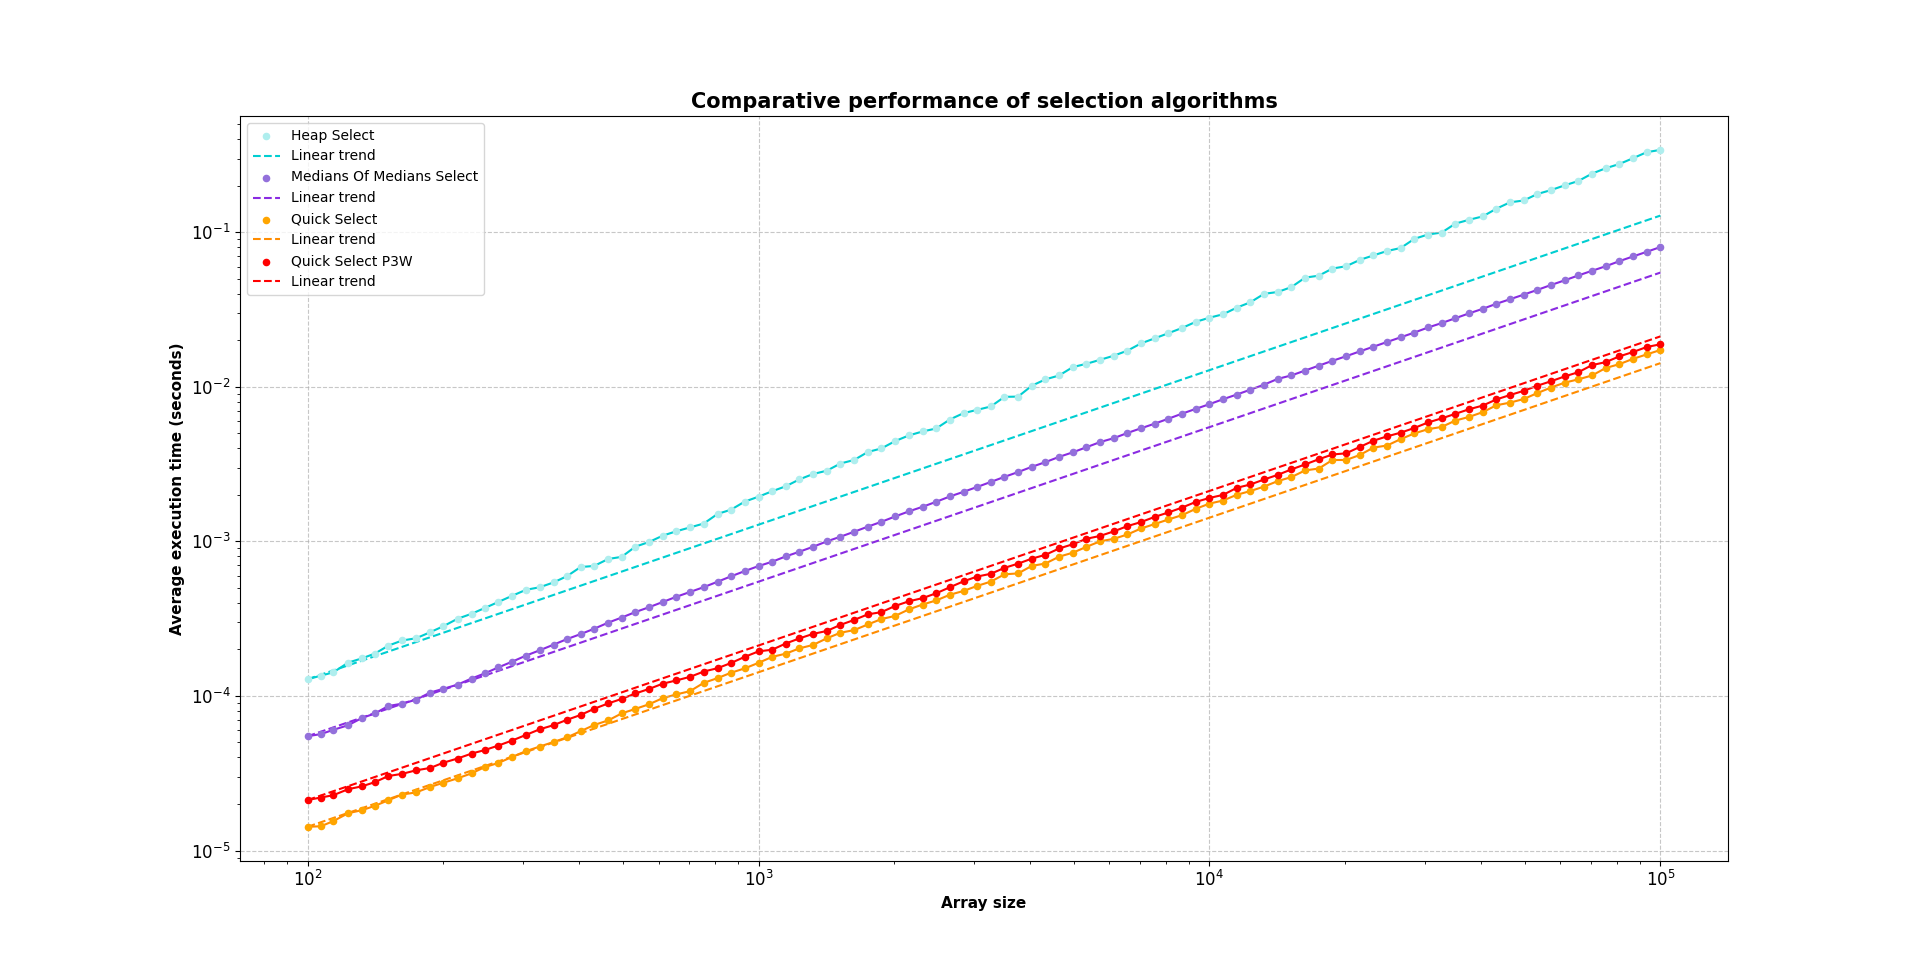
\includegraphics[width=1.2\textwidth]{Graphs/Final Graphs/kIsRandom_All_Log.png}
  }
  \caption{Comparative performance of selection algorithms - Logarithmic}
\end{figure}

\begin{figure}[H]   
  \makebox[\textwidth][c]{%
    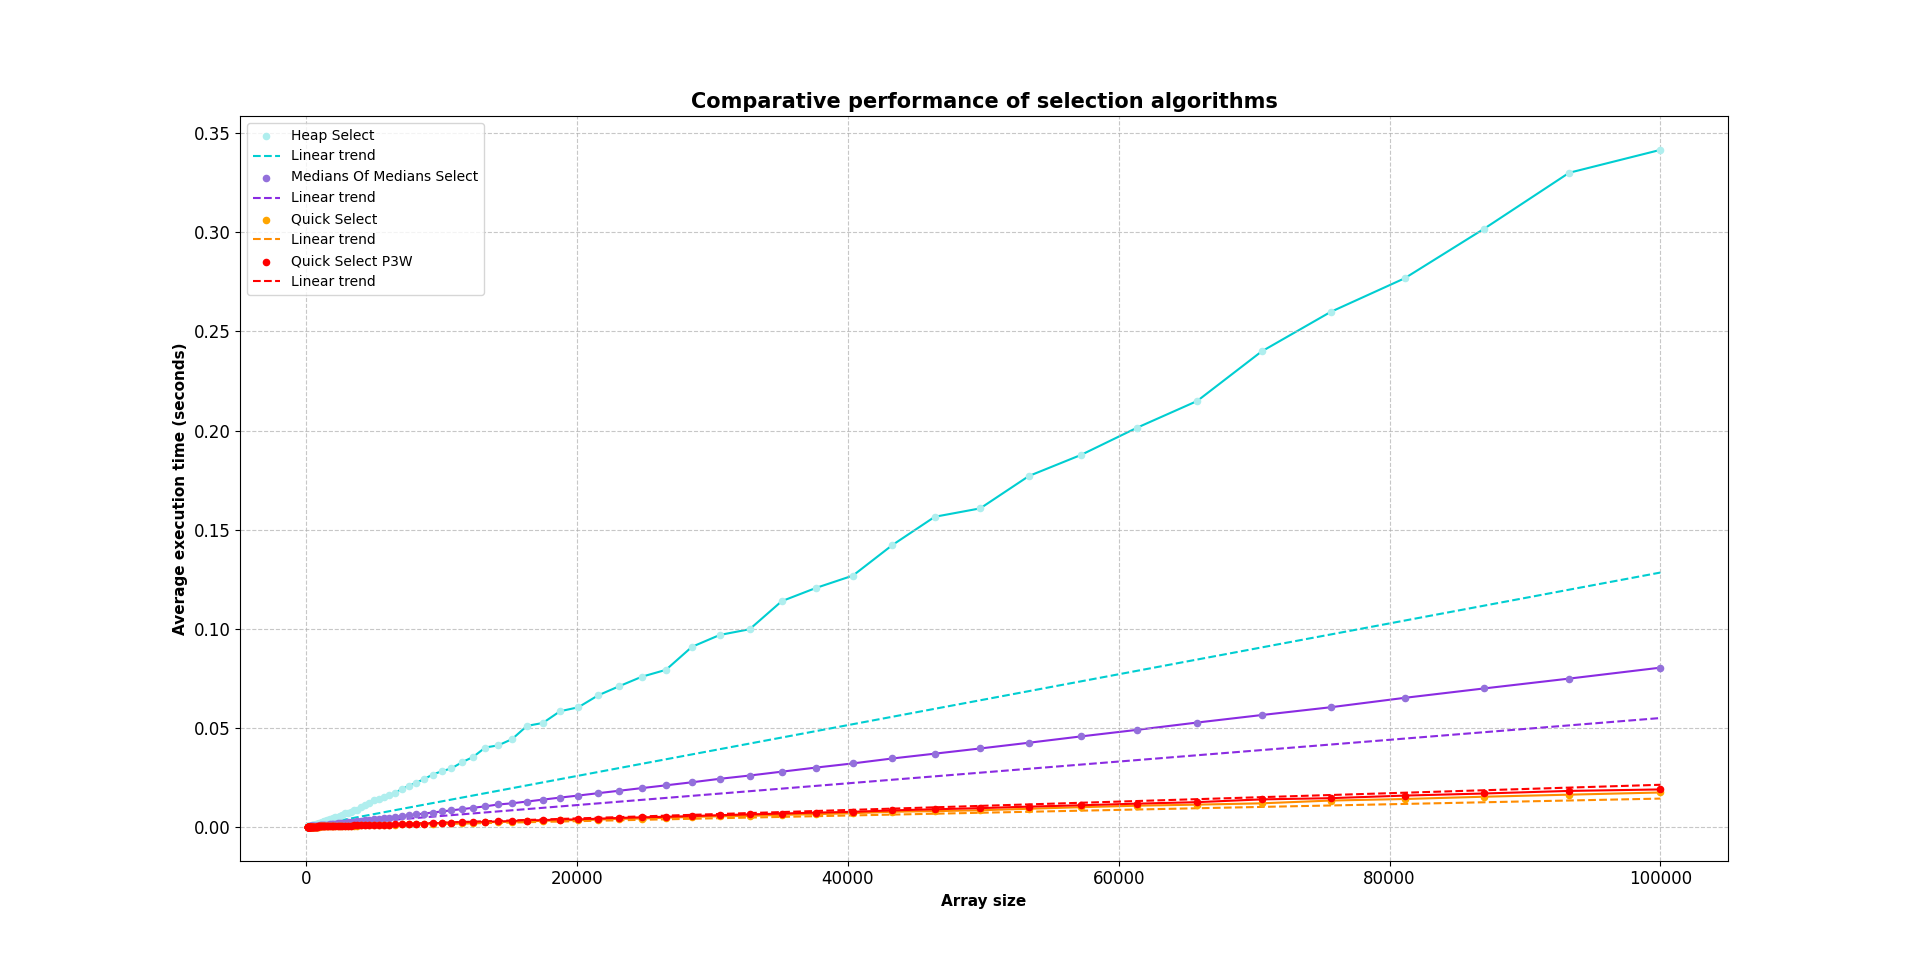
\includegraphics[width=1.2\textwidth]{Graphs/Final Graphs/kIsRandom_All_ notLog.png}
  }
  \caption{Comparative performance of selection algorithms - Linear}
\end{figure}

\section{Problems encountered and solutions found}
\begin{enumerate}
    \item When testing $QuickSelect$ in its worst case, with ordered arrays of more than 997 elements and $k=1$, the execution ended with a $'recursion depth'$ error because python could not compute all those recursions. We therefore transformed the recursive program into an iterative one. All the graphs in this report were generated by the iterative version.
    \item Initially, an integer key was used for $HeapSelect$ instead of a tuple [$element$, $position$] to represent a node. However, this caused 2 main problems:
    \begin{itemize}
        \item In case of repeated elements, a linear scan of the array was used to obtain the position of that key, which returned the position of the first occurrence of the specified element, thus only ever obtaining the children of the node that was needed first.\\
        This was solved by keeping track of the number of times the extracted keys appeared, with an occurrence map
        \item Having only the element keys available, we were forced to pass through each element of the array whenever we needed to find the position of one of them (to access its children).\\
        By using a tuple [$element$, $position$], the position of the children could be calculated immediately upon occurrence
    \end{itemize}
    \item Initially for the benchmark the idea was to save the data generated in an array to be passed to the function drawing the graph. However, we decided to save the data generated by the benchmark for each algorithm in separate files, just in case we wanted to:
    \begin{itemize}
        \item In case of repeated elements, a linear scan of the array was used to obtain the position of that key, which returned the position of the first occurrence of the specified element, thus only ever obtaining the children of the node that was needed first. This was solved by keeping track of the number of times the extracted keys appeared, with an occurrence map
        \item Having only the element keys available, we were forced to scroll through the array whenever we needed to find the position of one of them (to access its children). By using a tuple [$element$, $position$], the position of the children could be calculated immediately upon occurrence
    \end{itemize}
    \item The CPU of the MacBook Air, on which we ran the benchmark, reached rather high temperatures during the tests.\\
    Processor frequencies were also reduced and algorithm execution times increased more than expected with increasing array size until they stabilized from a certain point on.\\
    This, however, made the graphs inaccurate.\\
    This was a minor but easily avoidable distortion. We solved the problem by running the benchmark while holding the laptop over a running air conditioner in a university lecture hall.\\
    By combining the active dissipation provided by the air conditioner and the passive dissipation provided by the aluminium case, we greatly reduced the temperature and ensured more accurate results
\end{enumerate}

\section{Code}
All the code used in this report is available on this GitHub Repository: \\
https://github.com/NovaActias/ComparativeAnalysis-SelectionAlgorithms

\end{document}